%-------------------------------------------------------
%-- PREAMBLE
%-------------------------------------------------------
\documentclass[8pt]{beamer}
\usetheme[]{Feather}
  
\setbeamersize{text margin left=0.75cm,text margin right=0.75cm}

% INCLUDE PACKAGES
%-------------------------------------------------------

\usepackage[utf8]{inputenc}
\usepackage[english]{babel}
\usepackage[T1]{fontenc}
\usepackage{helvet}

\usepackage{graphicx}
\graphicspath{ {imgs/} }

\usepackage[utf8]{inputenc}
\usepackage[english]{babel}
\usepackage[protrusion=true,expansion=true]{microtype} 
\usepackage{amsmath,amsfonts,amsthm,amssymb,bm,mathdots,mathtools,bigints}
\usepackage{color, xcolor}
\usepackage{listings}
\usepackage[document]{ragged2e}
\usepackage{wrapfig}
\usepackage[printwatermark]{xwatermark}
\usepackage{subcaption}
\usepackage{mdframed}
\usepackage{multicol}
\usepackage{environ}
\usepackage{tikz, pgfplots}
\usepackage{framed}

\usepackage{biblatex}
\addbibresource{citations.bib}


\lstset{
    backgroundcolor=\color[rgb]{0.86,0.88,0.93},
    language=matlab, keywordstyle=\color[rgb]{0,0,1},
    basicstyle=\footnotesize \ttfamily,breaklines=true,
    escapeinside={\%*}{*)}
}

% DEFFINING COLORS
%-------------------------------------------------------
\definecolor{glgRed}{RGB}{214,45,32}
\definecolor{glgGreen}{RGB}{0,135,68}
\definecolor{glgBlue}{RGB}{0,87,231}
\definecolor{glgOrange}{RGB}{255,167,0}

\definecolor{retroBrown}{RGB}{102,101,71}
\definecolor{retroRed}{RGB}{251,46,1}
\definecolor{retroGreen}{RGB}{111,203,159}
\definecolor{retroYellow}{RGB}{255,226,138}

\definecolor{pastelBlue}{RGB}{27,133,184}
\definecolor{pastelRed}{RGB}{174,90,65}
\definecolor{pastelGreen}{RGB}{85,158,131}
\definecolor{pastelBlack}{RGB}{90,82,85}

\definecolor{niceBlack}{RGB}{14,17,17}
\definecolor{niceBlue}{RGB}{14,104,206}

\colorlet{signal1}{niceBlack!90}
\colorlet{signal2}{niceBlack!90}
\colorlet{signal3}{niceBlack!90}
\colorlet{signal4}{niceBlack!90}

% Beamer Color Scheme
\setbeamercolor{Feather}{fg=niceBlack!20,bg=pastelBlue!90}
\setbeamercolor{structure}{fg=niceBlack}
\setbeamercolor{frametitle}{bg=pastelBlue!70}
\setbeamercolor{normal text}{fg=black!85}


% Tikz Macros
% --------------------------------------------------------------------
\usetikzlibrary{shapes,arrows, backgrounds, positioning, fit, decorations.pathmorphing}

\tikzstyle{sectionBlock} = [draw, fill=blue!20, rectangle, minimum height=3em, minimum width=3em]
\tikzstyle{block} = [draw, fill=white, rectangle, minimum height=3em, minimum width=3em]
\tikzstyle{sum} = [draw, fill=white, circle, node distance=1cm]
\tikzstyle{input} = [coordinate]
\tikzstyle{output} = [coordinate]
\tikzstyle{pinstyle} = [pin edge={to-,thin,black}]
\tikzstyle{mcCircle} = [draw, circle, line width=0.5mm, minimum width=3em, minimum height=3em, fill=white]
\tikzstyle{mcInput} = [draw, rectangle, line width=0.5mm, minimum width=3em, minimum height=3em, fill=black!10]
\tikzstyle{mcCircleX} = [draw=glgBlue!80, circle, line width=0.75mm, minimum width=3em, minimum height=3em, fill=white]
\tikzstyle{mcCircleY} = [draw=glgBlue!80, circle, line width=0.75mm, minimum width=3em, minimum height=3em, fill=white]


% DEFFINING AND REDEFINING COMMANDS
%-------------------------------------------------------

% colored hyperlinks
\newcommand{\chref}[2]{
  \href{#1}{{\usebeamercolor[bg]{Feather}#2}}
}

\makeatletter
\let\beamer@writeslidentry@miniframeson=\beamer@writeslidentry
\def\beamer@writeslidentry@miniframesoff{%
  \expandafter\beamer@ifempty\expandafter{\beamer@framestartpage}{}% does not happen normally
  {%else
    % removed \addtocontents commands
    \clearpage\beamer@notesactions%
  }
}
\newcommand*{\miniframeson}{\let\beamer@writeslidentry=\beamer@writeslidentry@miniframeson}
\newcommand*{\miniframesoff}{\let\beamer@writeslidentry=\beamer@writeslidentry@miniframesoff}
\makeatother

\makeatletter
\patchcmd{\beamer@sectionintoc}
  {\vfill}
  {\vskip\itemsep}
  {}
  {}
\makeatother  

% tensor 2:
\newcommand{\tend}[1]{\hbox{\oalign{$\bm{#1}$\crcr\hidewidth$\scriptscriptstyle\bm{\sim}$\hidewidth}}}
\newcommand{\tenq}[1]{\hbox{\oalign{$\bm{#1}$\crcr\hidewidth$\scriptscriptstyle\bm{\sim}$\hidewidth}}}

%\let\oldfootnote\footnote
%\renewcommand\footnote[1][]{\oldfootnote[frame,#1]}

\let\oldFootnote\footnote
\newcommand\nextToken\relax

\let\oldFootfullcite\footfullcite

\renewcommand\footnote[1]{%
    \oldFootnote[frame]{#1}\futurelet\nextToken\isFootnote}

\newcommand\isFootnote{%
    \ifx\footnote\nextToken\textsuperscript{,}\fi}
    
\renewcommand\footfullcite[1]{%
  \oldFootfullcite{#1}\futurelet\nextToken\isFootfullcite}

\newcommand\isFootfullcite{%
    \ifx\footfullcite\nextToken\textsuperscript{,}\fi}

% ENVIROMENTS
%-------------------------------------------------------

\AtBeginSection[]{
  \begin{frame}
  \vfill
    \centering
    \Huge \color{niceBlack!85} \insertsectionhead\par%
  \vfill
  \end{frame}
}

%\AtBeginSubsection[]{
%  \begin{frame}
%  \vfill
%    \centering
%    \Huge \color{glgBlue!60} \insertsubsectionhead\par%
%    \huge \color{niceBlack!85} \insertsectionhead\par%
%  \vfill
%  \end{frame}
%}

\newenvironment<>{varblock}[2][.9\textwidth]{%
  \setlength{\textwidth}{#1}
  \begin{actionenv}#3%
    \def\insertblocktitle{#2}%
    \par%
    \usebeamertemplate{block begin}}
  {\par%
    \usebeamertemplate{block end}%
  \end{actionenv}}

\NewEnviron{myequation*}{%
    \begin{equation*}
    \scalebox{1.1}{$\BODY$}
    \end{equation*}
    }
    
% INFORMATION IN THE TITLE PAGE
%-------------------------------------------------------

\title[Optimal Control: An application to a non-isothermal continuous reactor]
{
      Optimal Control:\\An application to a non-isothermal continuous reactor
}

\subtitle[]
{
}

\author[Otacílio Bezerra Leite Neto]
{      
  Otacílio Bezerra Leite Neto\\
}

\institute[]
{
  TI0153 - Trabalho de Conclusão de Curso II\\
    Department of Teleinformatics Engineering\\
    Federal University of Ceará - UFC\\
  
  %there must be an empty line above this line - otherwise some unwanted space is added between the university and the country (I do not know why ;( )
}

\date{\today}

%-------------------------------------------------------
%-- THE BODY OF THE PRESENTATION
%-------------------------------------------------------

\begin{document}

%-------------------------------------------------------
% THE TITLEPAGE
%-------------------------------------------------------

{ \1
\begin{frame}[plain,noframenumbering] % the plain option removes the header from the title page, noframenumbering removes the numbering of this frame only
  \titlepage % call the title page information from above
\end{frame}}

%-------------------------------------------------------
% SUMMARY
%-------------------------------------------------------

\begin{frame}
  \setcounter{secnumdepth}{1}
  \setcounter{tocdepth}{1}
  \begin{center} \Large \bfseries
    Summary
  \end{center}
  \vfill
    \begin{columns}[t]
    	\hfill
        \begin{column}{0.4\textwidth}
            \tableofcontents[sections={1-3}]
        \end{column}
        \begin{column}{0.4\textwidth}
            \tableofcontents[sections={4-6}]
        \end{column}
        \hfill
    \end{columns}
\end{frame}


%-------------------------------------------------------
% SECTION - Introduction
%-------------------------------------------------------
\section{Introduction}
%-------------------------------------------------------
\subsection{Motivation}
%-------------------------------------------------------
\begin{frame}[c]{Introduction}{Contextualization}

\vskip0.25cm

\begin{itemize} \justifying
  \item<1-> We are discussing the \textbf{optimal control} of \textbf{dynamical systems}. \vskip0.2cm
  
  \item<2-> We are discussing \textbf{chemical reaction network systems}, for processes described as:\vskip0.2cm
  
  \begin{figure} \centering
    \resizebox{0.55\textwidth}{!}{\begin{tikzpicture}[auto, node distance=3cm, >=latex']
	\node [input] (input1) {};
	\node [input, below of=input1, node distance=1.5em] (input2) {};
	\node [input, below of=input2, node distance=1.5em] (input3) {};
	\node [block, right of=input2, minimum width=8em, minimum height=5em] (system) {{\large \bfseries System}};
	\node [output, right of=system] (output2) {};
	\node [output, above of=output2, node distance=1.5em] (output1) {};		
	\node [output, below of=output2, node distance=1.5em] (output3) {};
	
	\node [below of=system, node distance=6em] {$\left\{ \begin{matrix} \mathcal{R}^{(1)}  & \overset{K_{11}(T)}{\longrightarrow} & \cdots & \overset{K_{1n}(T)}{\longrightarrow} &  \mathcal{P}^{(1)} & & \Delta H_1 \\ \vdots &  & \vdots &  & \vdots  & &  \\ \mathcal{R}^{(N)} &  \overset{K_{n1}(T)}{\longrightarrow} & \cdots & \overset{K_{nn}(T)}{\longrightarrow} & \mathcal{P}^{(N)}  & & \Delta H_n \\ \end{matrix} \right.$};				
	
	\draw[->, line width=0.5mm] (input1) node[pos=0.1]{Reactants} -- (input1-|system.west);
	\draw[->, line width=0.5mm] (input3) -- node[pos=0.1]{Heat Capacity} (input3-|system.west);
	\draw[<-, line width=0.5mm] (output1) -- node[pos=0.1,yshift=1.5em]{Products} (output1-|system.east);
	\draw[<-, line width=0.5mm] (output3) -- node[pos=0.1,yshift=1.5em]{Temperature} (output3-|system.east);
\end{tikzpicture}}
  \end{figure} \vskip0cm
  
  \item<3-> Optimal control theory has been revisited from several innovative fields in the last years\footfullcite{Tang:2016}\footfullcite{Eren:2017}. Furthermore, reactor systems are subject of active research, with several open challenges. \footfullcite{Mulas:2015}
\end{itemize}

\end{frame}

%-------------------------------------------------------
\subsection{Problem Definition}
%-------------------------------------------------------
\begin{frame}[t]{Introduction}{Problem Definition}

\vskip0.25cm
\begin{itemize}
  \item The system used for the experiments was the \textit{non-isothermal Continuous Stirred Tank Reactor} (CSTR) presented by {\color{glgRed!50!black} [Klatt and Engell, 1998]}\footfullcite{Klatt:1998}. 
\end{itemize}

\begin{center}
\begin{varblock}[1\textwidth]{} \centering
  \includegraphics[width=0.5\textwidth]{exoCSTR}
\end{varblock}
\end{center} 

\end{frame}

%-------------------------------------------------------
\begin{frame}[t]{Introduction}{Problem Definition}
\addtocounter{footnote}{-1}

\vskip0.25cm
\begin{itemize}
  \item The system used for the experiments was the \textit{non-isothermal Continuous Stirred Tank Reactor} (CSTR) presented by {\color{glgRed!50!black} [Klatt and Engell, 1998]}\footfullcite{Klatt:1998}. 
\end{itemize} 

\begin{center}
\begin{varblock}[1\textwidth]{} \centering
  \begin{minipage}{.5\textwidth}
    \includegraphics[width=\textwidth]{exoCSTR}
  \end{minipage}%
  \begin{minipage}{.5\textwidth}
    {\justifying \bfseries This system...} \vskip0.2cm
    
    \begin{itemize} \justifying
      \item class of system that represents a wide range of industrial applications.\vskip0.2cm
      
      \item classical benchmark for multiple-input multiple-output (MIMO) control systems.\vskip0.2cm
      
      \item nonlinear behavior, models with non-minimum phase behavior and unmeasurable states.\vskip0.2cm
    \end{itemize}
  \end{minipage}
\end{varblock}
\end{center}

\end{frame}

%-------------------------------------------------------
% SECTION - Dynamical System Analysis
%-------------------------------------------------------
\section{Dynamical System Analysis}
%-------------------------------------------------------
\subsection{Dynamical Models for Chemical Reactors}
%-------------------------------------------------------
\begin{frame}[t]{Dynamical System Analysis}{Mathematical Models for Chemical Reactors}

\vskip0.25cm

We desire to obtain a State-Space mathematical representation of the system.
\begin{equation*}
\begin{cases}
  {\color{signal1} \dot{{\color{signal1} \bm{x}}}(t)} = {\color{signal2} \bm{f}(}{\color{signal1} {\color{signal1} \bm{x}}(t)}, {\color{signal1} {\color{signal1} \bm{u}}(t)} {\color{signal2} )} \\
    {\color{signal1} {\color{signal1} \bm{y}}(t)} = {\color{signal2} \bm{g}(}{\color{signal1} {\color{signal1} \bm{x}}(t)}, {\color{signal1} {\color{signal1} \bm{u}}(t)} {\color{signal2} )}
\end{cases}
\end{equation*} \vskip0.2cm

\begin{minipage}{\textwidth}
\begin{minipage}{0.45\textwidth}
\begin{itemize}
  \item[$\circ$] ${\color{signal1} {\color{signal1} \bm{x}}(t)} \in \mathbb{R}^n$ is the \textit{state-vector}.
  
  \item[$\circ$] ${\color{signal1} {\color{signal1} \bm{u}}(t)} \in \mathbb{R}^r$ is the \textit{input-vector}.
  
  \item[$\circ$] ${\color{signal1} {\color{signal1} \bm{y}}(t)} \in \mathbb{R}^p$ is the \textit{output-vector}.
\end{itemize}
\end{minipage}
\begin{minipage}{0.54\textwidth}
\begin{itemize}
  \item[$\circ$] ${\color{signal2} \bm{f}(\cdot)} : \mathbb{R}^{n\times r} \rightarrow \mathbb{R}^{n}$ is a \textit{state-transition function}.
  
  \item[$\circ$] ${\color{signal2} \bm{g}(\cdot)} : \mathbb{R}^{n\times r} \rightarrow \mathbb{R}^{p}$ is a \textit{output observation function}.
\end{itemize}
\end{minipage}
\end{minipage}

\vskip1cm
\begin{figure}[ht] \centering
    \resizebox{!}{!}{
    \begin{tikzpicture}[auto, node distance=2cm,>=latex', scale=0.2]
        % We start by placing the blocks
        \node [input, name=input] {};
        \node [block, fill=glgBlue!10, right of=input, minimum width=10em, minimum height=5em, node distance=9em] (system) {Open-Loop System};
        \node [output, right of=system, node distance=9em] (output) {};
        
        % Once the nodes are placed, connecting them is easy.       
        \draw [draw,->] (input) -- node[pos=0.1] {${\color{signal1} \bm{u}}$}  (system);
        \draw [->] (system) -- node[pos=0.9]{${\color{signal1} \bm{y}}$} (output);
        
    \end{tikzpicture}}
\end{figure}

\end{frame}

%-------------------------------------------------------
\begin{frame}[t]{Dynamical System Analysis}{Mathematical Models for Chemical Reactors}

\vskip0.25cm

We desire to obtain a State-Space mathematical representation of the system.
\begin{equation*}
\begin{cases}
  {\color{signal1} \dot{{\color{signal1} \bm{x}}}(t)} = {\color{signal2} \bm{A}}{\color{signal1} {\color{signal1} \bm{x}}(t)} + {\color{signal2} \bm{B}}{\color{signal1} {\color{signal1} \bm{u}}(t)} \\
    {\color{signal1} {\color{signal1} \bm{y}}(t)} = {\color{signal2} \bm{C}}{\color{signal1} {\color{signal1} \bm{x}}(t)} + {\color{signal2} \bm{D}}{\color{signal1} {\color{signal1} \bm{u}}(t)}
\end{cases}
\end{equation*} \vskip0.2cm

\begin{minipage}{\textwidth}
\begin{minipage}{0.47\textwidth}
\begin{itemize} \justifying
  \item[$\circ$] ${\color{signal1} {\color{signal1} \bm{x}}(t)} \in \mathbb{R}^n$ is the \textit{state-vector}.
  
  \item[$\circ$] ${\color{signal1} {\color{signal1} \bm{u}}(t)} \in \mathbb{R}^r$ is the \textit{input-vector}.
  
  \item[$\circ$] ${\color{signal1} {\color{signal1} \bm{y}}(t)} \in \mathbb{R}^p$ is the \textit{output-vector}.
\end{itemize}
\end{minipage}
\begin{minipage}{0.52\textwidth}
\begin{itemize} \justifying
  \item[$\circ$] ${\color{signal2} \bm{A}} \in \mathbb{R}^{n\times n}$ is the \textit{system matrix}.
  
  \item[$\circ$] ${\color{signal2} \bm{B}} \in \mathbb{R}^{n\times r}$ is the \textit{input matrix}.
  
  \item[$\circ$] ${\color{signal2} \bm{C}} \in \mathbb{R}^{p\times n}$ is the \textit{output matrix}.
  
  \item[$\circ$] ${\color{signal2} \bm{D}} \in \mathbb{R}^{p\times r}$ is the \textit{feedthrough matrix}.
\end{itemize}
\end{minipage}
\end{minipage}

\vskip0.1cm
\begin{figure}[ht]
    \centering
    \resizebox{!}{!}{
    \begin{tikzpicture}[auto, node distance=2cm,>=latex', scale=0.2]
        % We start by placing the blocks
        \node [input, name=input] {};
        \node [block, right of=input] (inputMatrix) {${\color{signal2} \bm{B}}$};
        \node [sum, right of=inputMatrix, node distance=4em] (stateSum) {};
        \node [block, right of=stateSum, node distance=4em] (integral) {$\int   $};
        \node [block, right of=integral, node distance=8em] (outputMatrix) {${\color{signal2} \bm{C}}$};
        \node [output, right of=outputMatrix] (output) {};
        \node [block, below of=integral, node distance=1.5cm] (stateMatrix) {${\color{signal2} \bm{A}}$};
        
        \begin{scope}[on background layer]
            \node [fit=(inputMatrix) (stateMatrix) (outputMatrix), fill= glgBlue!10, rounded corners, inner sep=.3cm, label={[xshift=3.7em, glgBlue!90]above left:Open-Loop System}] {};
        \end{scope}     
        
        % Once the nodes are placed, connecting them is easy.       
        \draw [draw,->] (input) -- node[pos=0.1] {${\color{signal1} \bm{u}}$} (inputMatrix);
        \draw [->] (inputMatrix) -- node[pos=0.8]{$+$} (stateSum);
        \draw [->] (stateSum) -- node[pos=0.5]{$\dot{{\color{signal1} \bm{x}}}$} (integral);
        \draw [->] (integral) -- node[name=bk1,pos=0.5]{} node[name=bk2,pos=0.5]{} node[pos=0.5]{${\color{signal1} \bm{x}}$} (outputMatrix);
        \draw [->] (outputMatrix) -- node[pos=0.9]{${\color{signal1} \bm{y}}$} (output);
        \draw [->] (bk1) |- (stateMatrix);
        \draw [->] (stateMatrix) -| node[pos=0.95]{$+$} (stateSum);
    \end{tikzpicture} 
    }
\end{figure}

\end{frame}

%-------------------------------------------------------
\begin{frame}[t]{Dynamical System Analysis}{Mathematical Models for Chemical Reactors}

\vskip0.25cm

We desire to obtain a State-Space mathematical representation of the system.
\begin{equation*}
\begin{cases}
  {\color{signal1} \dot{{\color{signal1} \bm{x}}}(t)} = {\color{signal2} \bm{A}}{\color{signal1} {\color{signal1} \bm{x}}(t)} + {\color{signal2} \bm{B}}{\color{signal1} {\color{signal1} \bm{u}}(t)} \\
    {\color{signal1} {\color{signal1} \bm{y}}(t)} = {\color{signal2} \bm{C}}{\color{signal1} {\color{signal1} \bm{x}}(t)} + {\color{signal2} \bm{D}}{\color{signal1} {\color{signal1} \bm{u}}(t)}
\end{cases}
\end{equation*} \vskip0.2cm

\textbf{This representation has several advantages.} \vskip0.2cm

\begin{itemize} \justifying
  \item<1-> The \textit{response} of the system has an analytical solution:
  \begin{equation*}
  \begin{cases}
        {\color{signal1} {\color{signal1} \bm{x}}(t)} = e^{{\color{signal2} \bm{A}}(t - t_0)} {\color{signal1} {\color{signal1} \bm{x}}(t)} + \displaystyle\int_{t_0}^{t} e^{{\color{signal2} \bm{A}}(t - \tau)} {\color{signal2} \bm{B}} {\color{signal1} {\color{signal1} \bm{u}}(\tau)} d \tau \hfill \\
        {\color{signal1} {\color{signal1} \bm{y}}(t)} = {\color{signal2} \bm{C}} e^{{\color{signal2} \bm{A}}(t - t_0)} {\color{signal1} {\color{signal1} \bm{x}}(t)} + {\color{signal2} \bm{C}} \displaystyle\int_{t_0}^{t} e^{{\color{signal2} \bm{A}}(t - \tau)} {\color{signal2} \bm{B}} {\color{signal1} {\color{signal1} \bm{u}}(\tau)} d \tau + {\color{signal2} \bm{D}} {\color{signal1} {\color{signal1} \bm{u}}(t)}
    \end{cases}
  \end{equation*} 
  
  \item<2|only@2> The \textit{stability} of the model is directly related to the eigenvalues ($\bm{\lambda}$) of ${\color{signal2} \bm{A}}$.
  \begin{equation*}
  \begin{matrix}
    {\color{signal1} {\color{signal1} \bm{x}}(t)} < \infty,\ {\color{signal1} t} \to \infty & \text{if } \text{Re}[\lambda_i] \leq 0,\ \forall i \in [1, n] 
  \end{matrix}
  \end{equation*}
  
  \item<3|only@3> The \textit{controllability} property is directly related to the \textit{Controllability Matrix}:
  \begin{equation*}
    \bm{\mathcal{C}} = \begin{bmatrix} {\color{signal2} \bm{B}} & {\color{signal2} \bm{A}} {\color{signal2} \bm{B}} & {\color{signal2} \bm{A}}^2 {\color{signal2} \bm{B}} & \cdots & {\color{signal2} \bm{A}}^{n-1} {\color{signal2} \bm{B}} \end{bmatrix}
  \end{equation*}
  
  \item<4|only@4> The \textit{observability} property is directly related to the \textit{Observability Matrix}:
  \begin{equation*}
    \bm{\mathcal{O}} = \begin{bmatrix} {\color{signal2} \bm{C}} & {\color{signal2} \bm{C}} {\color{signal2} \bm{A}} & {\color{signal2} \bm{C}} {\color{signal2} \bm{A}}^2  & \cdots & {\color{signal2} \bm{C}} {\color{signal2} \bm{A}}^{n-1} \end{bmatrix}^T
  \end{equation*}
\end{itemize}

\end{frame}

%-------------------------------------------------------
\begin{frame}[t]{Dynamical System Analysis}{Mathematical Models for Chemical Reactors}

\vskip0.25cm

\begin{varblock}[1\linewidth]{Linearization by Taylor Series Expansion}
  Consider a nonlinear time-invariant system:
    \begin{equation*} \label{eq:SSRepr03}
    \begin{cases}
  {\color{signal1} \dot{{\color{signal1} \bm{x}}}(t)} = {\color{signal2} \bm{f}(}{\color{signal1} {\color{signal1} \bm{x}}(t)}, {\color{signal1} {\color{signal1} \bm{u}}(t)} {\color{signal2} )} \\
    {\color{signal1} {\color{signal1} \bm{y}}(t)} = {\color{signal2} \bm{g}(}{\color{signal1} {\color{signal1} \bm{x}}(t)}, {\color{signal1} {\color{signal1} \bm{u}}(t)} {\color{signal2} )}
\end{cases}
    .\end{equation*}
    
    Given steady-state operating points ${\color{signal1} \bm{x}_o}$, ${\color{signal1} \bm{y}_o}$ and ${\color{signal1} \bm{u}_o}$, the dynamics of the system in the neighborhood of these points can be represented by the linear model: 
    \begin{align*}
    \begin{cases}
         { \color{signal1} \Delta \dot{{\color{signal1} \bm{x}}}(t)} = {\color{signal2} \bm{A}} { \color{signal1} \Delta {\color{signal1} \bm{x}}(t)} + {\color{signal2} \bm{B}} { \color{signal1} \Delta {\color{signal1} \bm{u}}(t)} & \\
        \hfill {\color{signal1} {\color{signal1} \bm{y}}(t)} = {\color{signal2} \bm{C}} { \color{signal1} \Delta {\color{signal1} \bm{x}}(t)} + {\color{signal2} \bm{D}} { \color{signal1} {\color{signal1} \Delta \bm{u}}(t)} &
    \end{cases}
    ,\end{align*}
    
    \noindent where
    \begin{equation*}
    \begin{matrix}
        {\color{signal2} \bm{A}} = \left. \cfrac{\partial {\color{signal2} \bm{f}}}{\partial {\color{signal1} \bm{x}}} \right|_{{\color{signal1} \bm{x}_o}, {\color{signal1} \bm{u}_o}}; & {\color{signal2} \bm{B}} = \left. \cfrac{\partial {\color{signal2} \bm{f}}}{\partial {\color{signal1} \bm{u}}} \right|_{{\color{signal1} \bm{x}_o}, {\color{signal1} \bm{u}_o}}; & {\color{signal2} \bm{C}} = \left. \cfrac{\partial {\color{signal2} \bm{g}}}{\partial {\color{signal1} \bm{x}}} \right|_{{\color{signal1} \bm{x}_o},  {\color{signal1} \bm{u}_o}}; & {\color{signal2} \bm{D}} = \left. \cfrac{\partial {\color{signal2} \bm{g}}}{\partial {\color{signal1} \bm{u}}} \right|_{{\color{signal1} \bm{x}_o}, {\color{signal1} \bm{u}_o}} 
    \end{matrix}
    \end{equation*}
    
    \noindent and
    \begin{equation*}
    \begin{matrix}
         {\color{signal1} \Delta {\color{signal1} \bm{x}}(t)} = {\color{signal1} {\color{signal1} \bm{x}}(t)} - {\color{signal1} \bm{x}_o}; & &  {\color{signal1} \Delta {\color{signal1} \bm{u}}(t)} = {\color{signal1} {\color{signal1} \bm{u}}(t)} - {\color{signal1} \bm{u}_o}
    \end{matrix}
    .\end{equation*}
\end{varblock}

\end{frame}

%-------------------------------------------------------
\subsection{First Principles Model Realization}
%-------------------------------------------------------
\begin{frame}[t]{Dynamical System Analysis}{First Principles Model Realization}

\vskip0.25cm

\begin{itemize}
  \item The first principle models are obtained through Conservation Laws from physics.
\end{itemize}

\begin{figure}
  \includegraphics[width=0.45\textwidth]{tank02}
\end{figure}
\begin{varblock}[1\linewidth]{Mass Balance for Chemical Compounds}
  \begin{equation*}
        \begin{pmatrix}
          \text{Accumulation} \\ \text{of mass} \\ \text{in the system}
      \end{pmatrix} =  \begin{pmatrix}
          \text{Mass flow} \\ \text{entering} \\ \text{system}
      \end{pmatrix} - \begin{pmatrix} \text{Mass flow} \\ \text{leaving} \\ \text{system}
      \end{pmatrix} \pm \begin{pmatrix}
          \text{Mass flow} \\ \text{from} \\ \text{reactions}
      \end{pmatrix}
    \end{equation*} \vskip0.2cm
\end{varblock}
  
\end{frame}

%-------------------------------------------------------
\begin{frame}[t]{Dynamical System Analysis}{Mathematical Models for Chemical Reactors}

\vskip0.25cm

\begin{itemize}
  \item The first principle models are obtained through Conservation Laws from physics.
\end{itemize}

\begin{figure}
  \includegraphics[width=0.45\textwidth]{tank02}
\end{figure}
\begin{varblock}[1\linewidth]{Mass Balance for Chemical Reactors}
  \begin{equation*}
        \cfrac{d (\rho_A)}{dt} = q (\rho^{(A)}_{in} - \rho^{(A)}_{out}) + \left( \sum_{\alpha X \rightarrow \beta A} \cfrac{1}{\beta} K_{XA}(T) (\rho_X)^{\alpha} \right) - \left(\sum_{\alpha A \rightarrow \beta X} \cfrac{1}{\beta} K_{AX}(T) (\rho_A)^{\alpha} \right)
    \end{equation*} \vskip0.2cm
\end{varblock}
  
\end{frame}

%-------------------------------------------------------
\begin{frame}[t]{Dynamical System Analysis}{Mathematical Models for Chemical Reactors}

\vskip0.25cm

\begin{itemize}
  \item The first principle models are obtained through Conservation Laws from physics.
\end{itemize}

\begin{figure}
  \includegraphics[width=0.45\textwidth]{tank02}
\end{figure}

\begin{varblock}[1\linewidth]{Conservation of Energy for Chemical Reactors}
  \begin{equation*}
        \begin{pmatrix}
            \text{Accumulation} \\ \text{of thermal energy} \\ \text{in the system}
        \end{pmatrix} = \begin{pmatrix}
            \text{Heat flow} \\ \text{entering} \\ \text{the system}
        \end{pmatrix} - \begin{pmatrix}
            \text{Heat flow} \\ \text{leaving} \\ \text{the system}
        \end{pmatrix} \pm \begin{pmatrix}
            \text{Entropy} \\ \text{contribution} \\ \text{from reactions}
        \end{pmatrix}
    \end{equation*} \vskip0.2cm
\end{varblock}
  
\end{frame}

%-------------------------------------------------------
\begin{frame}[t]{Dynamical System Analysis}{Mathematical Models for Chemical Reactors}

\vskip0.25cm

\begin{itemize}
  \item The first principle models are obtained through Conservation Laws from physics.
\end{itemize}

\begin{figure}
  \includegraphics[width=0.45\textwidth]{tank02}
\end{figure}

\begin{varblock}[1\linewidth]{Conservation of Energy for Chemical Reactors}
  \begin{equation*}
    \begin{cases}
        \cfrac{d(T)}{dt} = q(T_{in} - T_{out}) + \eta (T_C - T) + \delta \displaystyle\sum_{\alpha A \rightarrow \beta X} K_{AX}(T) (\rho_A)^{\alpha} \Delta H_{AX} \\
        \cfrac{d(T_C)}{dt} = \gamma Q + \beta (T - T_C)
    \end{cases}
    \end{equation*} \vskip0.2cm
\end{varblock}
  
\end{frame}

%%-------------------------------------------------------
\begin{frame}[t]{Dynamical System Analysis}{Mathematical Models for Chemical Reactors}

\vskip0.25cm

\begin{itemize}
  \item In the case of the reactor system in discussion, the model becomes...
\end{itemize}

\begin{varblock}[1\linewidth]{Mathematical Model of Non-Isothermal CSTR}
  \begin{equation*}
    \begin{cases}
  \hfill \cfrac{d(\rho_A)}{dt} &= q (\rho^{(A)}_{in} - \rho_A) - \left( K_1(T) \rho_A + K_3(T) \rho^2_A  \right) \\ \\
  \hfill \cfrac{d(\rho_B)}{dt} &= - q \rho_B + K_1(T) \rho_A - K_2(T) \rho_B \\ \\
  \hfill \cfrac{d(T)}{dt} &= q(T_{in} - T) + \cfrac{k_W A_r}{\varrho C_p V_r} (T_C - T) \\ & \ \ \ \ \ \ \ \ \ \ \ \ -\cfrac{1}{\varrho C_p} \left( K_1(T) \rho_A \Delta H_{AB} + K_2(T) \rho_B \Delta H_{BC} + K_1(T) \rho_A^2 \Delta H_{AC} \right) \\ \\
  \hfill \cfrac{d(T_C)}{dt} &= \cfrac{1}{m_K C_{pK}} Q + \cfrac{k_W A_r}{m_K C_{pK}} (T - T_C) 
\end{cases}
    \end{equation*} \vskip0.2cm
\end{varblock}

\end{frame}

%%-------------------------------------------------------
\begin{frame}[t]{Dynamical System Analysis}{Mathematical Models for Chemical Reactors}

\vskip0.25cm

\begin{itemize} \justifying
  \item We choose ${\color{signal1} \bm{x}} = [\rho_A, \rho_B, T, T_C]^T$, ${\color{signal1} \bm{u}} = [q, Q]^T$ and ${\color{signal1} \bm{y}} = [\rho_B, T]^T$. \vskip0.2cm
  
  \item We consider the steady-state point ${\color{signal1} \bm{x}_o} = [1.23, 0.90, 134.14, 128.95]^T$ and ${\color{signal1} \bm{u}_o} = [18.83, -4495.7]^T$.
\end{itemize}

\vskip0.5cm
\textbf{The linearized state-space model is described by matrices:}

\begin{varblock}[\textwidth]{}
\begin{equation*}
\left\{ \begin{matrix*}[l]
    {\color{signal1} \dot{{\color{signal1} \bm{x}}}(t)} = \begin{bmatrix*}[r]
      -86.1 &        0 &  -4.2 &        0 \\
       50.6 & -69.4 &   1.0 &        0 \\
      172.2 & 198.0 & -36.7 &  30.8 \\
             0 &       0  &  86.8 & -86.7
    \end{bmatrix*} \begin{bmatrix} {\color{signal1} x_1(t)} \\ {\color{signal1} x_2(t)} \\ {\color{signal1} x_3(t)} \\ {\color{signal1} x_4(t)} \end{bmatrix} + \begin{bmatrix*}[r] 
     3.9  &       0 \\
    -0.9  &       0 \\
    -4.1  &       0 \\
          0  &  0.1
    \end{bmatrix*} \begin{bmatrix} {\color{signal1} u_1(t)} \\ {\color{signal1} u_2(t)} \end{bmatrix} \hfill \\  \\ 
    {\color{signal1} \bm{y}} = \begin{bmatrix}
        0 & 1 & 0 & 0 \\ 0 & 0 & 1 & 0
    \end{bmatrix} \begin{bmatrix} {\color{signal1} x_1(t)} \\ {\color{signal1} x_2(t)} \\ {\color{signal1} x_3(t)} \\ {\color{signal1} x_4(t)} \end{bmatrix} + \begin{bmatrix}
        0 & 0 \\ 0 & 0
    \end{bmatrix} \begin{bmatrix} {\color{signal1} u_1(t)} \\ {\color{signal1} u_2(t)} \end{bmatrix} \hfill
\end{matrix*} \right.
\end{equation*}
\end{varblock}

\end{frame}

%%-------------------------------------------------------
\begin{frame}[t]{Dynamical System Analysis}{Mathematical Models for Chemical Reactors}

\vskip0.25cm
\textbf{The linearized state-space model is described by matrices:}

\begin{varblock}[\textwidth]{}
\begin{equation*}
\left\{ \begin{matrix*}[l]
    {\color{signal1} \dot{{\color{signal1} \bm{x}}}(t)} = \begin{bmatrix*}[r]
      -86.1 &        0 &  -4.2 &        0 \\
       50.6 & -69.4 &   1.0 &        0 \\
      172.2 & 198.0 & -36.7 &  30.8 \\
             0 &       0  &  86.8 & -86.7
    \end{bmatrix*} \begin{bmatrix} {\color{signal1} x_1(t)} \\ {\color{signal1} x_2(t)} \\ {\color{signal1} x_3(t)} \\ {\color{signal1} x_4(t)} \end{bmatrix} + \begin{bmatrix*}[r] 
     3.9  &       0 \\
    -0.9  &       0 \\
    -4.1  &       0 \\
          0  &  0.1
    \end{bmatrix*} \begin{bmatrix} {\color{signal1} u_1(t)} \\ {\color{signal1} u_2(t)} \end{bmatrix} \hfill \\  \\ 
    {\color{signal1} \bm{y}} = \begin{bmatrix}
        0 & 1 & 0 & 0 \\ 0 & 0 & 1 & 0
    \end{bmatrix} \begin{bmatrix} {\color{signal1} x_1(t)} \\ {\color{signal1} x_2(t)} \\ {\color{signal1} x_3(t)} \\ {\color{signal1} x_4(t)} \end{bmatrix} + \begin{bmatrix}
        0 & 0 \\ 0 & 0
    \end{bmatrix} \begin{bmatrix} {\color{signal1} u_1(t)} \\ {\color{signal1} u_2(t)} \end{bmatrix} \hfill
\end{matrix*} \right.
\end{equation*}
\end{varblock} \vskip0.2cm

\begin{itemize}
  \item<1|only@1> All the eigenvalues are real and negative. The system is \textbf{stable}.
  \begin{equation*}
    \bm{\lambda} = [-16.79, -54.84, -86.33, -121.01]
  \end{equation*}
  
  \item<2-> The Controllability Matrix has full-row rank. The system is \textbf{controllable}.
  \begin{equation*} 
    \texttt{rank}\left( \bm{\mathcal{C}} \right) = \texttt{rank}\left( \begin{bmatrix} {\color{signal2} \bm{B}} & {\color{signal2} \bm{A}} {\color{signal2} \bm{B}} & {\color{signal2} \bm{A}}^2 {\color{signal2} \bm{B}} & {\color{signal2} \bm{A}}^3 {\color{signal2} \bm{B}} \end{bmatrix} \right) = 4
  \end{equation*}
  
  \item<3-> The Observability Matrix has full-column rank. The system is \textbf{observable}.
  \begin{equation*} 
    \texttt{rank}\left( \bm{\mathcal{O}} \right) = \texttt{rank}\left( \begin{bmatrix} {\color{signal2} \bm{C}} & {\color{signal2} \bm{C}} {\color{signal2} \bm{A}} & {\color{signal2} \bm{C}} {\color{signal2} \bm{A}}^2 & {\color{signal2} \bm{C}} {\color{signal2} \bm{A}}^3 \end{bmatrix} \right) = 4
  \end{equation*}
\end{itemize}

\end{frame}

%-------------------------------------------------------
\subsection{Experiments}
%-------------------------------------------------------
\begin{frame}[c]{Dynamical System Analysis}{Experiments}

\vskip0.25cm

\begin{figure}[ht] \centering
    \begin{tikzpicture} [node distance=1cm]
    \node (plot) {\includegraphics[width=\textwidth]{dynamics04}};
    
    \begin{scope}[on background layer]
      \node[block, minimum height=1.75em, above of=plot, xshift=0.45cm, node distance=2.75cm, minimum width=0.7\textwidth] (legendBox) {};
    \end{scope}
    
    \definecolor{linecolor}{rgb}{0, 0.4470, 0.7410};
    \node at (legendBox.west) [xshift=0.4cm]  (legendStart) {};
    \node[right of=legendStart, node distance=1cm] (label) {$\rho_A$};    
    \draw[-, linecolor, line width=1pt] (legendStart) -- (label);
    
    \definecolor{linecolor}{rgb}{0.8500,0.3250,0.0980};
    \node[right of=label]  (legendStart) {};
    \node[right of=legendStart, node distance=1cm] (label) {$\rho_B$};    
    \draw[-, linecolor, line width=1pt] (legendStart) -- (label);
    
    \definecolor{linecolor}{rgb}{0.6350, 0.0780, 0.1840};
    \node[right of=label]  (legendStart) {};
    \node[right of=legendStart, node distance=1cm] (label) {$T$};   
    \draw[-, linecolor, line width=1pt] (legendStart) -- (label);
    
    \definecolor{linecolor}{rgb}{0.3010, 0.7450, 0.9330};
    \node[right of=label]  (legendStart) {};
    \node[right of=legendStart, node distance=1cm] (label) {$T_c$};   
    \draw[-, linecolor, line width=1pt] (legendStart) -- (label);
  \end{tikzpicture} 
\end{figure}

\end{frame}

%-------------------------------------------------------
\begin{frame}[c]{Dynamical System Analysis}{Experiments}

\vskip0.25cm

\begin{figure}[ht] \centering
    \begin{tikzpicture} [node distance=1cm]
    \node (plot) {\includegraphics[width=\textwidth]{linear01}};
    
    \begin{scope}[on background layer]
      \node[block, minimum height=1.75em, above of=plot, xshift=0.45cm, node distance=2.75cm, minimum width=0.7\textwidth] (legendBox) {};
    \end{scope}
    
    \definecolor{linecolor}{rgb}{0, 0.4470, 0.7410};
    \node at (legendBox.west) [xshift=0.4cm]  (legendStart) {};
    \node[right of=legendStart, node distance=1cm] (label) {$\rho_A$};    
    \draw[-, linecolor, line width=1pt] (legendStart) -- (label);
    
    \definecolor{linecolor}{rgb}{0.8500,0.3250,0.0980};
    \node[right of=label]  (legendStart) {};
    \node[right of=legendStart, node distance=1cm] (label) {$\rho_B$};    
    \draw[-, linecolor, line width=1pt] (legendStart) -- (label);
    
    \definecolor{linecolor}{rgb}{0.6350, 0.0780, 0.1840};
    \node[right of=label]  (legendStart) {};
    \node[right of=legendStart, node distance=1cm] (label) {$T$};   
    \draw[-, linecolor, line width=1pt] (legendStart) -- (label);
    
    \definecolor{linecolor}{rgb}{0.3010, 0.7450, 0.9330};
    \node[right of=label]  (legendStart) {};
    \node[right of=legendStart, node distance=1cm] (label) {$T_c$};   
    \draw[-, linecolor, line width=1pt] (legendStart) -- (label);
  \end{tikzpicture} 
\end{figure}

\end{frame}


%-------------------------------------------------------
% SECTION - State-Feedback Controllers
%-------------------------------------------------------
\section{State-Feedback Controllers}
%-------------------------------------------------------
\subsection{Definitions}
%-------------------------------------------------------
\begin{frame}[t]{State-Feedback Controllers}{Definitions}

\vskip0.25cm

\begin{varblock}[1\linewidth]{Full State-Feedback Controller}
      The input action ${\color{signal1} {\color{signal1} \bm{u}}(t)}$ is calculated by the linear control law $\pi(\cdot)$ through state-feedback as:
    \begin{equation*}
        {\color{signal1} {\color{signal1} \bm{u}}(t)} = \pi({\color{signal1} {\color{signal1} \bm{r}}(t)}, {\color{signal1} {\color{signal1} \bm{x}}(t)}) = {\color{signal1} {\color{signal1} \bm{r}}(t)} - {\color{signal4} \bm{K}} {\color{signal1} {\color{signal1} \bm{x}}(t)}
    ,\end{equation*}
    
    \noindent where ${\color{signal1} \bm{r}} : \mathbb{R} \rightarrow \mathbb{R}^{n}$ is a state reference signal and ${\color{signal4} \bm{K}} \in \mathbb{R}^{r \times n}$ is the \textit{feedback gain matrix}.
\end{varblock} \vskip0.2cm

\begin{itemize}
  \item<1|only@1> Substituting this control law to the model results in the closed-loop representation:
  \begin{equation*}
  \begin{split}
    {\color{signal1} \dot{{\color{signal1} \bm{x}}}(t)} &= {\color{signal2} \bm{A}}{\color{signal1} {\color{signal1} \bm{x}}(t)} + {\color{signal2} \bm{B}}( {\color{glgBlue!90} {\color{signal1} {\color{signal1} \bm{r}}(t)}} - {\color{signal4} \bm{K}} {\color{signal1} {\color{signal1} \bm{x}}(t)}) \\
    &= ({\color{signal2} \bm{A}} - {\color{signal2} \bm{B}}{\color{signal4} \bm{K}}) {\color{signal1} {\color{signal1} \bm{x}}(t)} + {\color{signal2} \bm{B}}{\color{glgBlue!90} {\color{signal1} {\color{signal1} \bm{r}}(t)}} \\
    &= {\color{signal2} {\color{signal2} \bm{A}}_{cl}} {\color{signal1} {\color{signal1} \bm{x}}(t)} + {\color{signal2} \bm{B}}{\color{glgBlue!90} {\color{signal1} {\color{signal1} \bm{r}}(t)}} 
  \end{split}
  \end{equation*}

  \item<2|only@2>[] \begin{figure}[ht]
      \centering
      \resizebox{0.8\textwidth}{!}{
        \begin{tikzpicture}[auto, node distance=1.8cm,>=latex', scale=0.2]
            % We start by placing the blocks
            \node [input, name=input] {};
            \node [sum, right of=input, node distance=4em] (fbckSum) {};
            \node [block, right of=fbckSum] (inputMatrix) {${\color{signal2} \bm{B}}$};
            \node [sum, right of=inputMatrix, node distance=4em] (stateSum) {};
            \node [block, right of=stateSum, node distance=4em] (integral) {$\int   $};
            \node [block, right of=integral, node distance=8em] (outputMatrix) {${\color{signal2} \bm{C}}$};
            \node [output, right of=outputMatrix] (output) {};
            \node [block, below of=integral, node distance=1.5cm] (stateMatrix) {${\color{signal2} \bm{A}}$};
            \node [block, below of=stateSum, node distance=10em, label={below:Controller}] (fbckGain) {${\color{signal4} \bm{K}}$};
            
            \begin{scope}[on background layer]
                \node [fit=(inputMatrix) (stateMatrix) (outputMatrix), fill= glgBlue!10, rounded corners, inner sep=.3cm, label={[xshift=3.75em, glgBlue!90]above left:Open-Loop System}] {};
            \end{scope}     
            
            % Once the nodes are placed, connecting them is easy.       
            \draw [draw,->] (input) -- node[pos=0.1] {${\color{signal1} \bm{r}}$} node[pos=0.8] {$+$}  (fbckSum);
            \draw [->] (fbckSum) -- node[pos=0.3]{${\color{signal1} \bm{u}}$} (inputMatrix);
            \draw [->] (inputMatrix) -- node[pos=0.8]{$+$} (stateSum);
            \draw [->] (stateSum) -- node[pos=0.5]{$\dot{{\color{signal1} \bm{x}}}$} (integral);
            \draw [->] (integral) -- node[name=bk1,pos=0.5]{} node[name=bk2,pos=0.5]{} node[pos=0.5]{${\color{signal1} \bm{x}}$} (outputMatrix);
            \draw [->] (outputMatrix) -- node[pos=0.6]{${\color{signal1} \bm{y}}$} (output);
            \draw [->] (bk1) |- (stateMatrix);
            \draw [->] (bk2) |- (fbckGain);
            \draw [->] (stateMatrix) -| node[pos=0.95]{$+$} (stateSum);
            \draw [->] (fbckGain) -| node[pos=0.97]{$-$} (fbckSum);
        \end{tikzpicture} 
        }
  \end{figure}
    
  \item<3-> Substituting this control law to the model results in the closed-loop representation:
    \begin{equation*}
    \begin{split}
      {\color{signal1} \dot{{\color{signal1} \bm{x}}}(t)} &= {\color{signal2} \bm{A}}{\color{signal1} {\color{signal1} \bm{x}}(t)} + {\color{signal2} \bm{B}}( {\color{glgBlue!90} {\color{signal1} {\color{signal1} \bm{r}}(t)}} - {\color{signal4} \bm{K}} {\color{signal1} {\color{signal1} \bm{x}}(t)}) \\
      &= ({\color{signal2} \bm{A}} - {\color{signal2} \bm{B}}{\color{signal4} \bm{K}}) {\color{signal1} {\color{signal1} \bm{x}}(t)} + {\color{signal2} \bm{B}}{\color{glgBlue!90} {\color{signal1} {\color{signal1} \bm{r}}(t)}} \\
      &= {\color{signal2} {\color{signal2} \bm{A}}_{cl}} {\color{signal1} {\color{signal1} \bm{x}}(t)} + {\color{signal2} \bm{B}}{\color{glgBlue!90} {\color{signal1} {\color{signal1} \bm{r}}(t)}} 
    \end{split}
    \end{equation*} \vskip0.2cm
  
  \item<3-> \textbf{Pole-Placement Property:} If $({\color{signal2} \bm{A}}, {\color{signal2} \bm{B}})$ is \textit{controllable}, we can assign the eigenvalues of ${\color{glgRed!80} {\color{signal2} \bm{A}_{cl}}}$ anywhere in the complex plane by means of designing ${\color{signal4} \bm{K}}$.
\end{itemize}

\end{frame}

%-------------------------------------------------------
\subsection{Regulation vs. Tracking}
%-------------------------------------------------------
\begin{frame}[t]{State-Feedback Controllers}{Regulation vs. Tracking}

\vskip0.4cm
{\justifying \textbf{We discuss the two modes of operation for state-feedback controllers.}}

\vskip0.5cm
\begin{minipage}{\textwidth}
\begin{minipage}{0.47\textwidth}
\begin{varblock}[\textwidth]{}
  \begin{center} \textbf{Regulation} \end{center}
  
  \begin{itemize} \justifying
    \item \textbf{Objective:} maintain the system in some position (the zero-state) and reject disturbances. \vskip0.25cm
    
    \item Special case of the state-feedback when ${\color{signal1} {\color{signal1} \bm{r}}(t)} = 0$. \vskip0.25cm
    
    \item Direct from the controller formulation. \vskip0.25cm
  \end{itemize}\vskip0.25cm
\end{varblock}
\end{minipage}
\hfill
\begin{minipage}{0.47\textwidth}
\end{minipage}
\end{minipage}

\end{frame}

%-------------------------------------------------------
\begin{frame}[t]{State-Feedback Controllers}{Regulation vs. Tracking}

\vskip0.4cm
{\justifying \textbf{We discuss the two modes of operation for state-feedback controllers.}}

\vskip0.5cm
\begin{minipage}{\textwidth}
\begin{minipage}{0.47\textwidth}
\begin{varblock}[\textwidth]{}
  \begin{center} \textbf{Regulation} \end{center}
  
  \begin{itemize} \justifying
    \item \textbf{Objective:} maintain the system in some position (the zero-state) and reject disturbances. \vskip0.25cm
    
    \item Special case of the state-feedback when ${\color{signal1} {\color{signal1} \bm{r}}(t)} = 0$. \vskip0.25cm
    
    \item Direct from the controller formulation. \vskip0.25cm
  \end{itemize}\vskip0.25cm
\end{varblock}
\end{minipage}
\hfill
\begin{minipage}{0.47\textwidth}
\begin{varblock}[\textwidth]{}
  \begin{center} \textbf{Reference Tracking} \end{center}
  
  \begin{itemize} \justifying
    \item \textbf{Objective:} drive the states of the system towards a non-constant reference signal. \vskip0.25cm
    
    \item Special case of the state-feedback when ${\color{signal1} {\color{signal1} \bm{r}}(t)}$ is non-constant. \vskip0.25cm
    
    \item Raises the need for \textit{integral action}. \vskip0.25cm
  \end{itemize}\vskip0.25cm
\end{varblock}
\end{minipage}
\end{minipage}

\end{frame}

%-------------------------------------------------------
\begin{frame}[t]{State-Feedback Controllers}{Regulation vs. Tracking}

\vskip0.4cm
{\justifying \textbf{We discuss the two modes of operation for state-feedback controllers.}}

\vskip0.2cm
\begin{varblock}[\textwidth]{State-Feedback with Integral Action}
  Consider a State-space system and augmented state ${\color{signal1} \bm{x}}_a : \mathbb{R} \rightarrow \mathbb{R}^{p}$ defined by:
    \begin{equation*}
        {\color{signal1} \bm{x}_a(t)} = \int_{0}^{t} \left( {\color{signal1} \bm{r}}(\tau) - {\color{signal1} \bm{y}}(\tau) \right) d\tau \Longrightarrow {\color{signal1} \dot{{\color{signal1} \bm{x}}}_a(t)} = {\color{signal1} {\color{signal1} \bm{r}}(t)} - {\color{signal1} {\color{signal1} \bm{y}}(t)}
    .\end{equation*}
    
\noindent A robust tracking (or servo) controller, defined by the gain $\tilde{{\color{signal4} \bm{K}}} = \begin{bmatrix} {\color{signal4} \bm{K}} & {\color{signal4} \bm{K}}_a \end{bmatrix}$, for ${\color{signal4} \bm{K}} \in \mathbb{R}^{r \times n}$ and ${\color{signal4} \bm{K}}_a \in \mathbb{R}^{r \times p}$, operates on the following augmented version of the original system:
    \begin{align*} \label{eq:augmentedSystem}
    \begin{cases}
        \begin{bmatrix}
            {\color{signal1} \dot{{\color{signal1} \bm{x}}}(t)} \\
            {\color{signal1} \dot{{\color{signal1} \bm{x}_a(t)}}}
        \end{bmatrix} &= \begin{bmatrix}
            {\color{signal2} \bm{A}} - {\color{signal2} \bm{B}} {\color{signal4} \bm{K}} & -{\color{signal2} \bm{B}} {\color{signal4} \bm{K}}_a \\ - {\color{signal2} \bm{C}} & \bm{0}
        \end{bmatrix} \begin{bmatrix}
            {\color{signal1} {\color{signal1} \bm{x}}(t)} \\
            {\color{signal1} \bm{x}_a(t)}
        \end{bmatrix} + \begin{bmatrix}
            \bm{0} \\
            \bm{I_p}
        \end{bmatrix} {\color{signal1} {\color{signal1} \bm{r}}(t)}
        \\
        \hfill {\color{signal1} {\color{signal1} \bm{y}}(t)} &= \begin{bmatrix}
            {\color{signal2} \bm{C}} & \bm{0}
        \end{bmatrix} \begin{bmatrix}
            {\color{signal1} {\color{signal1} \bm{x}}(t)} \\
            {\color{signal1} \bm{x}_a(t)}
        \end{bmatrix}
    \end{cases}
    .\end{align*} \vskip0.25cm
\end{varblock}

\end{frame}

%-------------------------------------------------------
\begin{frame}[c]{State-Feedback Controllers}{Regulation vs. Tracking}

\begin{figure}[ht]
    \centering
    \resizebox{\textwidth}{!}{
    \begin{tikzpicture}[auto, node distance=1.8cm,>=latex']
        % We start by placing the blocks
        \node [input, name=input] {};
        \node [sum, right of=input, node distance=4em] (intFbckSum) {};
        \node [block, right of=intFbckSum, node distance=4em] (integralAction) {$\int$};
        \node [block, right of=integralAction, node distance=6em] (intActGain) {${\color{signal4} \bm{K}}_a$};
        \node [sum, right of=intActGain, node distance=4.5em] (fbckSum) {};
        \node [block, right of=fbckSum] (inputMatrix) {${\color{signal2} \bm{B}}$};
        \node [sum, right of=inputMatrix, node distance=4em] (stateSum) {};
        \node [block, right of=stateSum, node distance=4em] (integral) {$\int   $};
        \node [block, right of=integral, node distance=8em] (outputMatrix) {${\color{signal2} \bm{C}}$};
        \node [output, right of=outputMatrix] (output) {};
        \node [block, below of=integral] (stateMatrix) {${\color{signal2} \bm{A}}$};
        \node [block, below of=stateSum, node distance=13em, label={below:Controller}] (fbckGain) {${\color{signal4} \bm{K}}$};
        
        \begin{scope}[on background layer]
            \node [fit=(inputMatrix) (stateMatrix) (outputMatrix), fill= glgBlue!10, rounded corners, inner sep=.4cm, label={[xshift=3.5em, glgBlue!90]above left:Open-Loop System}] {};
        \end{scope}     
        
        \begin{scope}[on background layer]
            \node [fit=(integralAction) (intActGain), fill= glgGreen!10, rounded corners, inner sep=.4cm, label={[xshift=4.3em, glgGreen!90]above left:Integral Action}] {};
        \end{scope} 
        
        % Once the nodes are placed, connecting them is easy.       
        \draw [draw,->] (input) -- node[pos=0.1] {${\color{signal1} \bm{r}}$} node[pos=0.8] {$+$}  (intFbckSum);
        \draw [->] (intFbckSum) -- (integralAction);
        \draw [->] (integralAction) -- node[pos=0.5]{${\color{signal1} \bm{x}}_a$} (intActGain);
        \draw [->] (intActGain) -- node[pos=0.8]{$-$} (fbckSum);
        \draw [->] (fbckSum) -- node[pos=0.3]{${\color{signal1} \bm{u}}$} (inputMatrix);
        \draw [->] (inputMatrix) -- node[pos=0.8]{$+$} (stateSum);
        \draw [->] (stateSum) -- node[pos=0.5]{$\dot{{\color{signal1} \bm{x}}}$} (integral);
        \draw [->] (integral) -- node[name=bk1,pos=0.5]{} node[name=bk2,pos=0.5]{} node[pos=0.5]{${\color{signal1} \bm{x}}$} (outputMatrix);
        \draw [->] (outputMatrix) -- node[name=bk3,pos=0.5]{} node[pos=0.6]{${\color{signal1} \bm{y}}$} (output);
        \draw [->] (bk1) |- (stateMatrix);
        \draw [->] (bk2) |- (fbckGain);
        \draw [->] (stateMatrix) -| node[pos=0.95]{$+$} (stateSum);
        \draw [->] (fbckGain) -| node[pos=0.97]{$-$} (fbckSum);
        \draw [->] (bk3) -- ++(0, -17em) -| node[pos=0.97]{$-$} (intFbckSum);
    \end{tikzpicture} 
    }
\end{figure}

\end{frame}

%-------------------------------------------------------
% SECTION - Optimal Control
%-------------------------------------------------------
\section{Optimal Control}
%-------------------------------------------------------
\subsection{Formulation}
%-------------------------------------------------------
\begin{frame}[t]{Optimal Control}{Formulation}

\vskip0.25cm

\begin{varblock}[1\linewidth]{Optimal Controller - General Formulation} \justifying
  The input action ${\color{signal1} \bm{u}}  (t) \in \mathbb{R}^r$ is \textit{optimal} if an \textit{optimal control law} $\pi^* : \mathbb{R}^{n \times n \times 1} \rightarrow \mathbb{R}^r$ can be found as:
      \begin{equation*}
          {\color{signal1} {\color{signal1} \bm{u}}(t)} = \pi^*({\color{signal1} \bm{x}}, {\color{signal1} \bm{r}}, t) = \operatorname*{arg\,min}_{{\color{signal1} \bm{u}}} J({\color{signal1} \bm{x}}, {\color{signal1} \bm{r}}, t)
      ,\end{equation*}
      
  \noindent where $J : \mathbb{R}^{n \times n \times 1} \rightarrow \mathbb{R}$ is known as the \textit{cost function}. \vskip0.2cm
\end{varblock} \vskip0.5cm

\begin{itemize}
  \item<1-> \textbf{This is still a state-feedback controller}: the cost function is a function of past values of the state and reference signals. \vskip0.25cm
  
  \item<2-> Reduces the need for hand-designing the feedback gain or any other control law for the system, given some specifications. \vskip0.25cm
  
  \item<3-> The type of the optimal controller depends on the choice of $J(\cdot)$ and (possibly) on how the optimization is solved. \vskip0.25cm
\end{itemize}

\end{frame}

%-------------------------------------------------------
\begin{frame}[t]{Optimal Control}{Formulation}

\vskip0.25cm

\begin{varblock}[1\linewidth]{Finite-Horizon Optimal Regulators}
  A \textit{Finite-Horizon Optimal Regulator} is defined as any controller whose optimal policy over a time interval $t \in [t_0, T]$ minimizes the cost functional:
    \begin{equation*}
        J({\color{signal1} \bm{x}}, {\color{signal1} \bm{u}}, t_0) = \int_{t_0}^T l({\color{signal1} \bm{x}}, {\color{signal1} \bm{u}}, \tau) d \tau + l_f({\color{signal1} \bm{x}}, T)
    ,\end{equation*}
    
    \noindent where $l(\cdot) : \mathbb{R}^{n \times r \times 1} \rightarrow \mathbb{R}$ and $l_f(\cdot) : \mathbb{R}^{n} \rightarrow \mathbb{R}$ are, respectively, the \textit{trajectory} and \textit{terminal loss functions}. In the case that $t_0 = 0$, $T$ is also known as the \textit{control horizon}.
\end{varblock} \vskip0.4cm

\begin{itemize}
  \item<1-> \textbf{Regulator:} this class of optimal controllers is defined for ${\color{signal1} {\color{signal1} \bm{r}}(t)} = \bm{0}$. \vskip0.2cm
  
  \item<2-> If $l({\color{signal1} \bm{x}}, {\color{signal1} \bm{u}}, \tau) \geq 0$ and $l_f({\color{signal1} \bm{x}}, T) \geq 0$, $\forall {\color{signal1} \bm{x}}, {\color{signal1} \bm{u}}, \tau$, then the cost function penalizes deviations from the zero-state.
  
  \item<3-> Characterizes an entire class of optimal controllers based on finite horizon optimization.
\end{itemize}

\end{frame}

%-------------------------------------------------------
\begin{frame}[t]{Optimal Control}{Formulation}

\vskip0.25cm

\begin{varblock}[1\linewidth]{Hamilton-Jacobi-Bellman (HJB) equation} \justifying
  Consider a finite-horizon cost function for a system described by $\dot{{\color{signal1} \bm{x}}} = \bm{f}({\color{signal1} \bm{x}}, {\color{signal1} \bm{u}}, t)$:
    \begin{equation*} \label{eq:valueCostFunctional}
      V({\color{signal1} \bm{x}}, {\color{signal1} \bm{u}}, t_0) = \int_{t_0}^T l({\color{signal1} \bm{x}}, {\color{signal1} \bm{u}}, \tau) d \tau + l_f({\color{signal1} \bm{x}}(T))
    \end{equation*}
    
    \noindent Minimizing any functional in the form of $V(\cdot)$ is equivalent to determining the solution of the \textit{Hamilton-Jacobi equation*}:
    \begin{equation*} \label{eq:HJequation*}
        \cfrac{\partial V^*}{\partial t} = - \min_{u(t)} \left[ l({\color{signal1} \bm{x}}, {\color{signal1} \bm{u}}, t) + \left[ \cfrac{\partial V^*}{\partial x} \right]^T \bm{f}({\color{signal1} \bm{x}}, {\color{signal1} \bm{u}}, t)  \right]
    \end{equation*}
    
    \noindent and the boundary condition:
    \begin{equation*}
        V^*({\color{signal1} \bm{x}}, T) = l_f({\color{signal1} \bm{x}}(T))
    .\end{equation*} \vskip0.2cm
\end{varblock}

\end{frame}

%-------------------------------------------------------
\begin{frame}[c]{Optimal Control}{Formulation}

\vskip0.25cm

\begin{itemize}
  \item The HJB equation provides a \textit{sufficient condition} for finite-horizon optimal controllers. \vskip0.2cm
  
  \item This class of optimal controllers is related to the \textit{Bellman's Principle of Optimality}. \vskip0.2cm
\end{itemize}

\begin{figure}[ht] \centering
    \resizebox{0.6\textwidth}{!}{
    \begin{tikzpicture}[auto, node distance=1.75cm,>=latex', scale=0.2]
        % Nodes
        \node [mcCircle] (x0) {$x_0$};
        
        \node [mcCircle, right of=x0, node distance=12em] (x12) {};
        \node [mcCircle, above of=x12] (x11) {};
        \node [mcCircle, below of=x12] (x13) {};
        
        \node [mcCircle, right of=x12, node distance=14em] (xT) {$x_T$};
        
        % Scopes
        \begin{scope}[on background layer]
            \node [fit=(x11) (x13), fill= black!10, rounded corners, inner sep=.4cm, label={[xshift=0em, black!90]above:$x_1$}] {};
        \end{scope}         
        
        % Lines
        \draw [->, color=glgRed!80, line width=.75mm] (x0) -- node[pos=0.7]{$70$} (x11);
        \draw [->] (x0) -- node[pos=0.6]{$40$} (x12);
        \draw [->] (x0) -- node[pos=0.45]{$130$} (x13);
        
        \draw [->, color=glgRed!80, line width=.75mm, decorate, decoration={snake,amplitude=1.5mm, segment length=8mm}] (x11) -- node[pos=0.31]{$220$} (xT);
        \draw [->, decorate, decoration={snake,amplitude=1.5mm, segment length=8mm}] (x12) -- node[pos=0.48]{$270$} (xT);
        \draw [->, decorate, decoration={snake,amplitude=1.5mm, segment length=8mm}] (x13) -- node[pos=0.53]{$190$} (xT);
    \end{tikzpicture} 
    }
\end{figure}

\end{frame}


%-------------------------------------------------------
\subsection{Linear Quadratic (LQ) Controllers}
%-------------------------------------------------------
\begin{frame}[t]{Optimal Control}{Linear Quadratic (LQ) Controllers}

\vskip0.25cm

\begin{varblock}[1\linewidth]{Linear Quadratic Regulator (LQR)}
  Given a linear State-Space system in the form:
    \begin{align*}
    \begin{cases}
        {\color{signal1} \dot{{\color{signal1} \bm{x}}}(t)} = {\color{signal2} \bm{A}} {\color{signal1} {\color{signal1} \bm{x}}(t)} + {\color{signal2} \bm{B}} {\color{signal1} {\color{signal1} \bm{u}}(t)} \\
        {\color{signal1} {\color{signal1} \bm{y}}(t)} = {\color{signal2} \bm{C}} {\color{signal1} {\color{signal1} \bm{x}}(t)} + {\color{signal2} \bm{D}} {\color{signal1} {\color{signal1} \bm{u}}(t)}
    \end{cases}
    .\end{align*}
    
    A \textit{Linear Quadratic Regulator} (LQR) for this system is an optimal controller defined by the quadratic cost function:
    \begin{equation*}
        J({\color{signal1} \bm{x}}, {\color{signal1} \bm{u}}, t_0) = \int_{t_0}^{T} \left( {\color{signal1} \bm{x}}^T {\color{signal3} \bm{Q}} {\color{signal1} \bm{x}} + {\color{signal1} \bm{u}}^T {\color{signal3} \bm{R}} {\color{signal1} \bm{u}} \right) dt + {\color{signal1} \bm{x}}^T(T) {\color{signal3} \bm{Q}}_f {\color{signal1} \bm{x}}(T)
    ,\end{equation*}
    
    \noindent where is assumed that ${\color{signal3} \bm{Q}},{\color{signal3} \bm{Q}}_f  \succ 0$ and ${\color{signal3} \bm{R}} \succ 0$.
\end{varblock} \vskip0.2cm

\begin{itemize}
  \item<1-> Defined for a \textit{linear} system with \textit{quadratic} cost function. \vskip0.2cm
  
  \item<2-> The weights ${\color{signal3} \bm{Q}}$, ${\color{signal3} \bm{Q}}_f$ and ${\color{signal3} \bm{R}}$ are chosen to reflect how the designer wish to penalize state-deviation or control effort. \vskip0.2cm
  
  \item<3-> \textbf{Optimization:} closed-form solution for $\pi^*({\color{signal1} \bm{x}}, {\color{signal1} \bm{u}}, t_0)$. \vskip0.2cm
\end{itemize}

\end{frame}

%-------------------------------------------------------
\begin{frame}[t]{Optimal Control}{Linear Quadratic (LQ) Controllers}

\vskip0.25cm

\begin{varblock}[1\linewidth]{LQR Control Action from Dynamic Programming}
  Given a Linear Quadratic Regulator, the optimal action produced is given by:
    \begin{equation*}
        {\color{signal1} {\color{signal1} \bm{u}}^*(t)} = - {\color{signal3} \bm{R}}^{-1} {\color{signal2} \bm{B}}^T {\color{signal3} \bm{P}}(t) {\color{signal1} {\color{signal1} \bm{x}}(t)}
    ,\end{equation*}
    
    \noindent where ${\color{signal3} \bm{P}}(t)$ is the solution of the matrix Riccati differential equation:
    \begin{equation*}
        -\dot{{\color{signal3} \bm{P}}}(t) = {\color{signal2} \bm{A}}^T {\color{signal3} \bm{P}}(t) + {\color{signal3} \bm{P}}(t) {\color{signal2} \bm{A}} - {\color{signal3} \bm{P}}(t) {\color{signal2} \bm{B}} {\color{signal3} \bm{R}}^{-1} {\color{signal2} \bm{B}}^T {\color{signal3} \bm{P}}(t) + {\color{signal3} \bm{Q}}
    ,\end{equation*}
    
    \noindent with terminal condition ${\color{signal3} \bm{P}}(T) = {\color{signal3} \bm{Q}}_f$.
\end{varblock} \vskip0.3cm

\begin{itemize} \justifying
  \item<1|only@1> Notice that:
  \begin{equation*}
    \begin{split}
      {\color{signal1} \dot{{\color{signal1} \bm{x}}}(t)} &= {\color{signal2} \bm{A}}{\color{signal1} {\color{signal1} \bm{x}}(t)} + {\color{signal2} \bm{B}}{\color{glgBlue!90} {\color{signal1} {\color{signal1} \bm{u}}^*(t)}} \\
      &= {\color{signal2} \bm{A}}{\color{signal1} {\color{signal1} \bm{x}}(t)} + {\color{signal2} \bm{B}}(- {\color{signal3} \bm{R}}^{-1} {\color{signal2} \bm{B}}^T {\color{signal3} \bm{P}}(t) {\color{signal1} {\color{signal1} \bm{x}}(t)}) \\
      &= ({\color{signal2} \bm{A}} - {\color{signal2} \bm{B}} {\color{signal3} \bm{R}}^{-1} {\color{signal2} \bm{B}}^T {\color{signal3} \bm{P}}(t)) {\color{signal1} {\color{signal1} \bm{x}}(t)} \\
      &= ({\color{signal2} \bm{A}} - {\color{signal2} \bm{B}} {\color{glgRed!80} {\color{signal4} \bm{K}(t)}}) {\color{signal1} {\color{signal1} \bm{x}}(t)} \\
    \end{split}
  \end{equation*} \vskip0.2cm
  
  \item<2-> The optimization results in a \textit{linear} and \textit{time-varying} control law:
  \begin{equation*}
    {\color{signal1} {\color{signal1} \bm{u}}^*(t)} = \pi^*({\color{signal1} \bm{x}}, {\color{signal1} \bm{u}}, t) = {\color{signal1} {\color{signal1} \bm{r}}(t)} - {\color{signal4} \bm{K}(t)} {\color{signal1} {\color{signal1} \bm{x}}(t)}
  \end{equation*}
  
  \item<3-> \textbf{``Open-Loop" Optimization:} the matrix ${\color{signal4} \bm{K}(t)}$ does not depend on past (or actual) states. The Ricatti differential equation can be solved off-line.
  
  \item<4-> \textbf{Remark:} nevertheless, the optimal controller performs corrective action.
\end{itemize}

\end{frame}

%-------------------------------------------------------
\begin{frame}[t]{Optimal Control}{Linear Quadratic (LQ) Controllers}

\vskip0.25cm

\begin{varblock}[1\linewidth]{LQR with Integral Action}
  Given a linear State-Space system augmented with state ${\color{signal1} \dot{{\color{signal1} \bm{x}}}_a(t)} = {\color{signal1} {\color{signal1} \bm{r}}(t)} - {\color{signal2} \bm{C}} {\color{signal1} {\color{signal1} \bm{x}}(t)}$:
    \begin{align*} 
    \begin{cases}
        \begin{bmatrix}
            {\color{signal1} \dot{{\color{signal1} \bm{x}}}(t)} \\
            {\color{signal1} \dot{{\color{signal1} \bm{x}}}_a(t)}
        \end{bmatrix} &= \underbrace{\begin{bmatrix}
            {\color{signal2} \bm{A}}  & \bm{0} \\ - {\color{signal2} \bm{C}} & \bm{0}
        \end{bmatrix}}_{\tilde{{\color{signal2} \bm{A}}}} \underbrace{\begin{bmatrix}
            {\color{signal1} {\color{signal1} \bm{x}}(t)} \\
            {\color{signal1} \bm{x}}_a(t)
        \end{bmatrix}}_{\tilde{{\color{signal1} \bm{x}}}(t)} + \underbrace{\begin{bmatrix}
            {\color{signal2} \bm{B}} \\
            \bm{0}
        \end{bmatrix}}_{\tilde{{\color{signal2} \bm{B}}}} {\color{signal1} {\color{signal1} \bm{u}}(t)} + \begin{bmatrix}
            \bm{0} \\
            \bm{I}
        \end{bmatrix} {\color{signal1} {\color{signal1} \bm{r}}(t)}
        \\
        \hfill {\color{signal1} {\color{signal1} \bm{y}}(t)} &= \begin{bmatrix}
            {\color{signal2} \bm{C}} & \bm{0}
        \end{bmatrix} \begin{bmatrix}
            {\color{signal1} {\color{signal1} \bm{x}}(t)} \\
            {\color{signal1} \bm{x}}_a(t)
        \end{bmatrix}
    \end{cases}
    .\end{align*}
    
    A \textit{Linear Quadratic Servo} (LQ-Servo) for this system is an optimal controller defined by the quadratic cost function:
    \begin{equation*}
        J({\color{signal1} \bm{x}}, {\color{signal1} \bm{u}}, t_0) = \int_{t_0}^{T} \left( \tilde{{\color{signal1} \bm{x}}}^T \tilde{{\color{signal3} \bm{Q}}} \tilde{{\color{signal1} \bm{x}}} + {\color{signal1} \bm{u}}^T {\color{signal3} \bm{R}} {\color{signal1} \bm{u}} \right) dt +\tilde{{\color{signal1} \bm{x}}} \tilde{{\color{signal3} \bm{Q}}}_f \tilde{{\color{signal1} \bm{x}}}(T)
    ,\end{equation*}
    
    \noindent where is assumed that $\tilde{{\color{signal3} \bm{Q}}}, \tilde{{\color{signal3} \bm{Q}}}_f \succ 0$ and ${\color{signal3} \bm{R}} \succ 0$.
\end{varblock}

\end{frame}

%-------------------------------------------------------
\subsection{Simulations}
%-------------------------------------------------------
\begin{frame}[c]{Optimal Control}{Simulations}

\vskip0.25cm

\begin{figure}[h]
  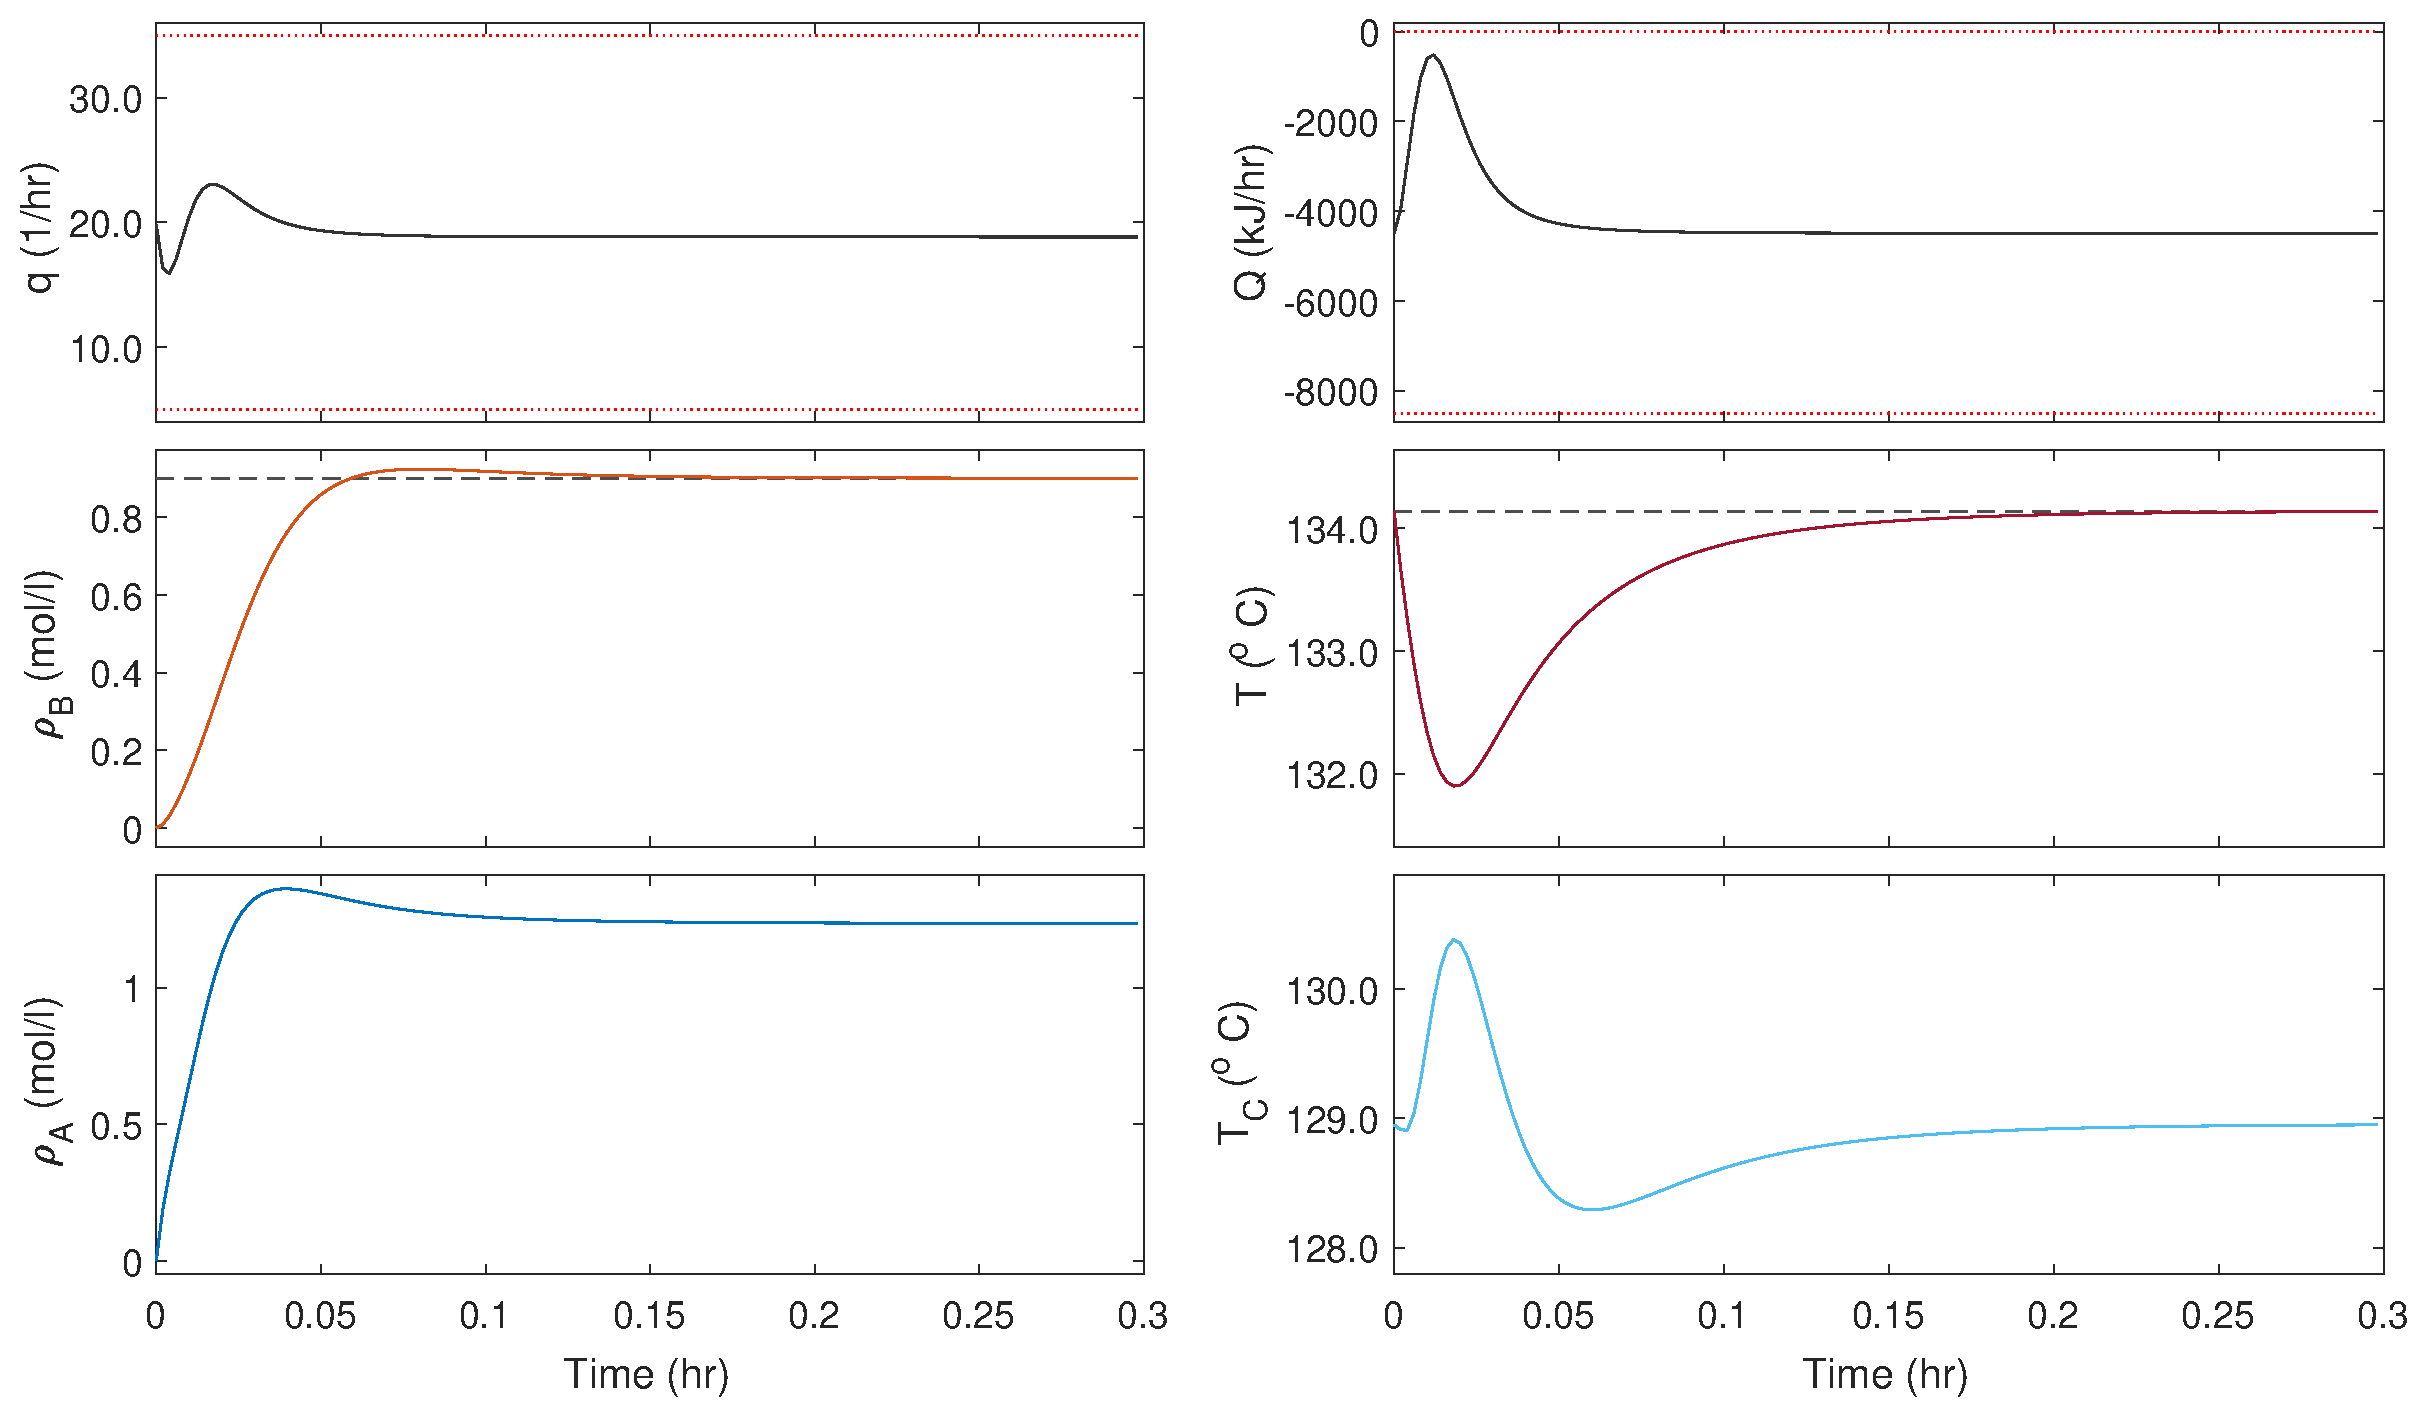
\includegraphics[width=\textwidth]{lqr01}
\end{figure}

\end{frame}

%-------------------------------------------------------
\begin{frame}[c]{Optimal Control}{Simulations}

\vskip0.25cm

\begin{figure}[h]
  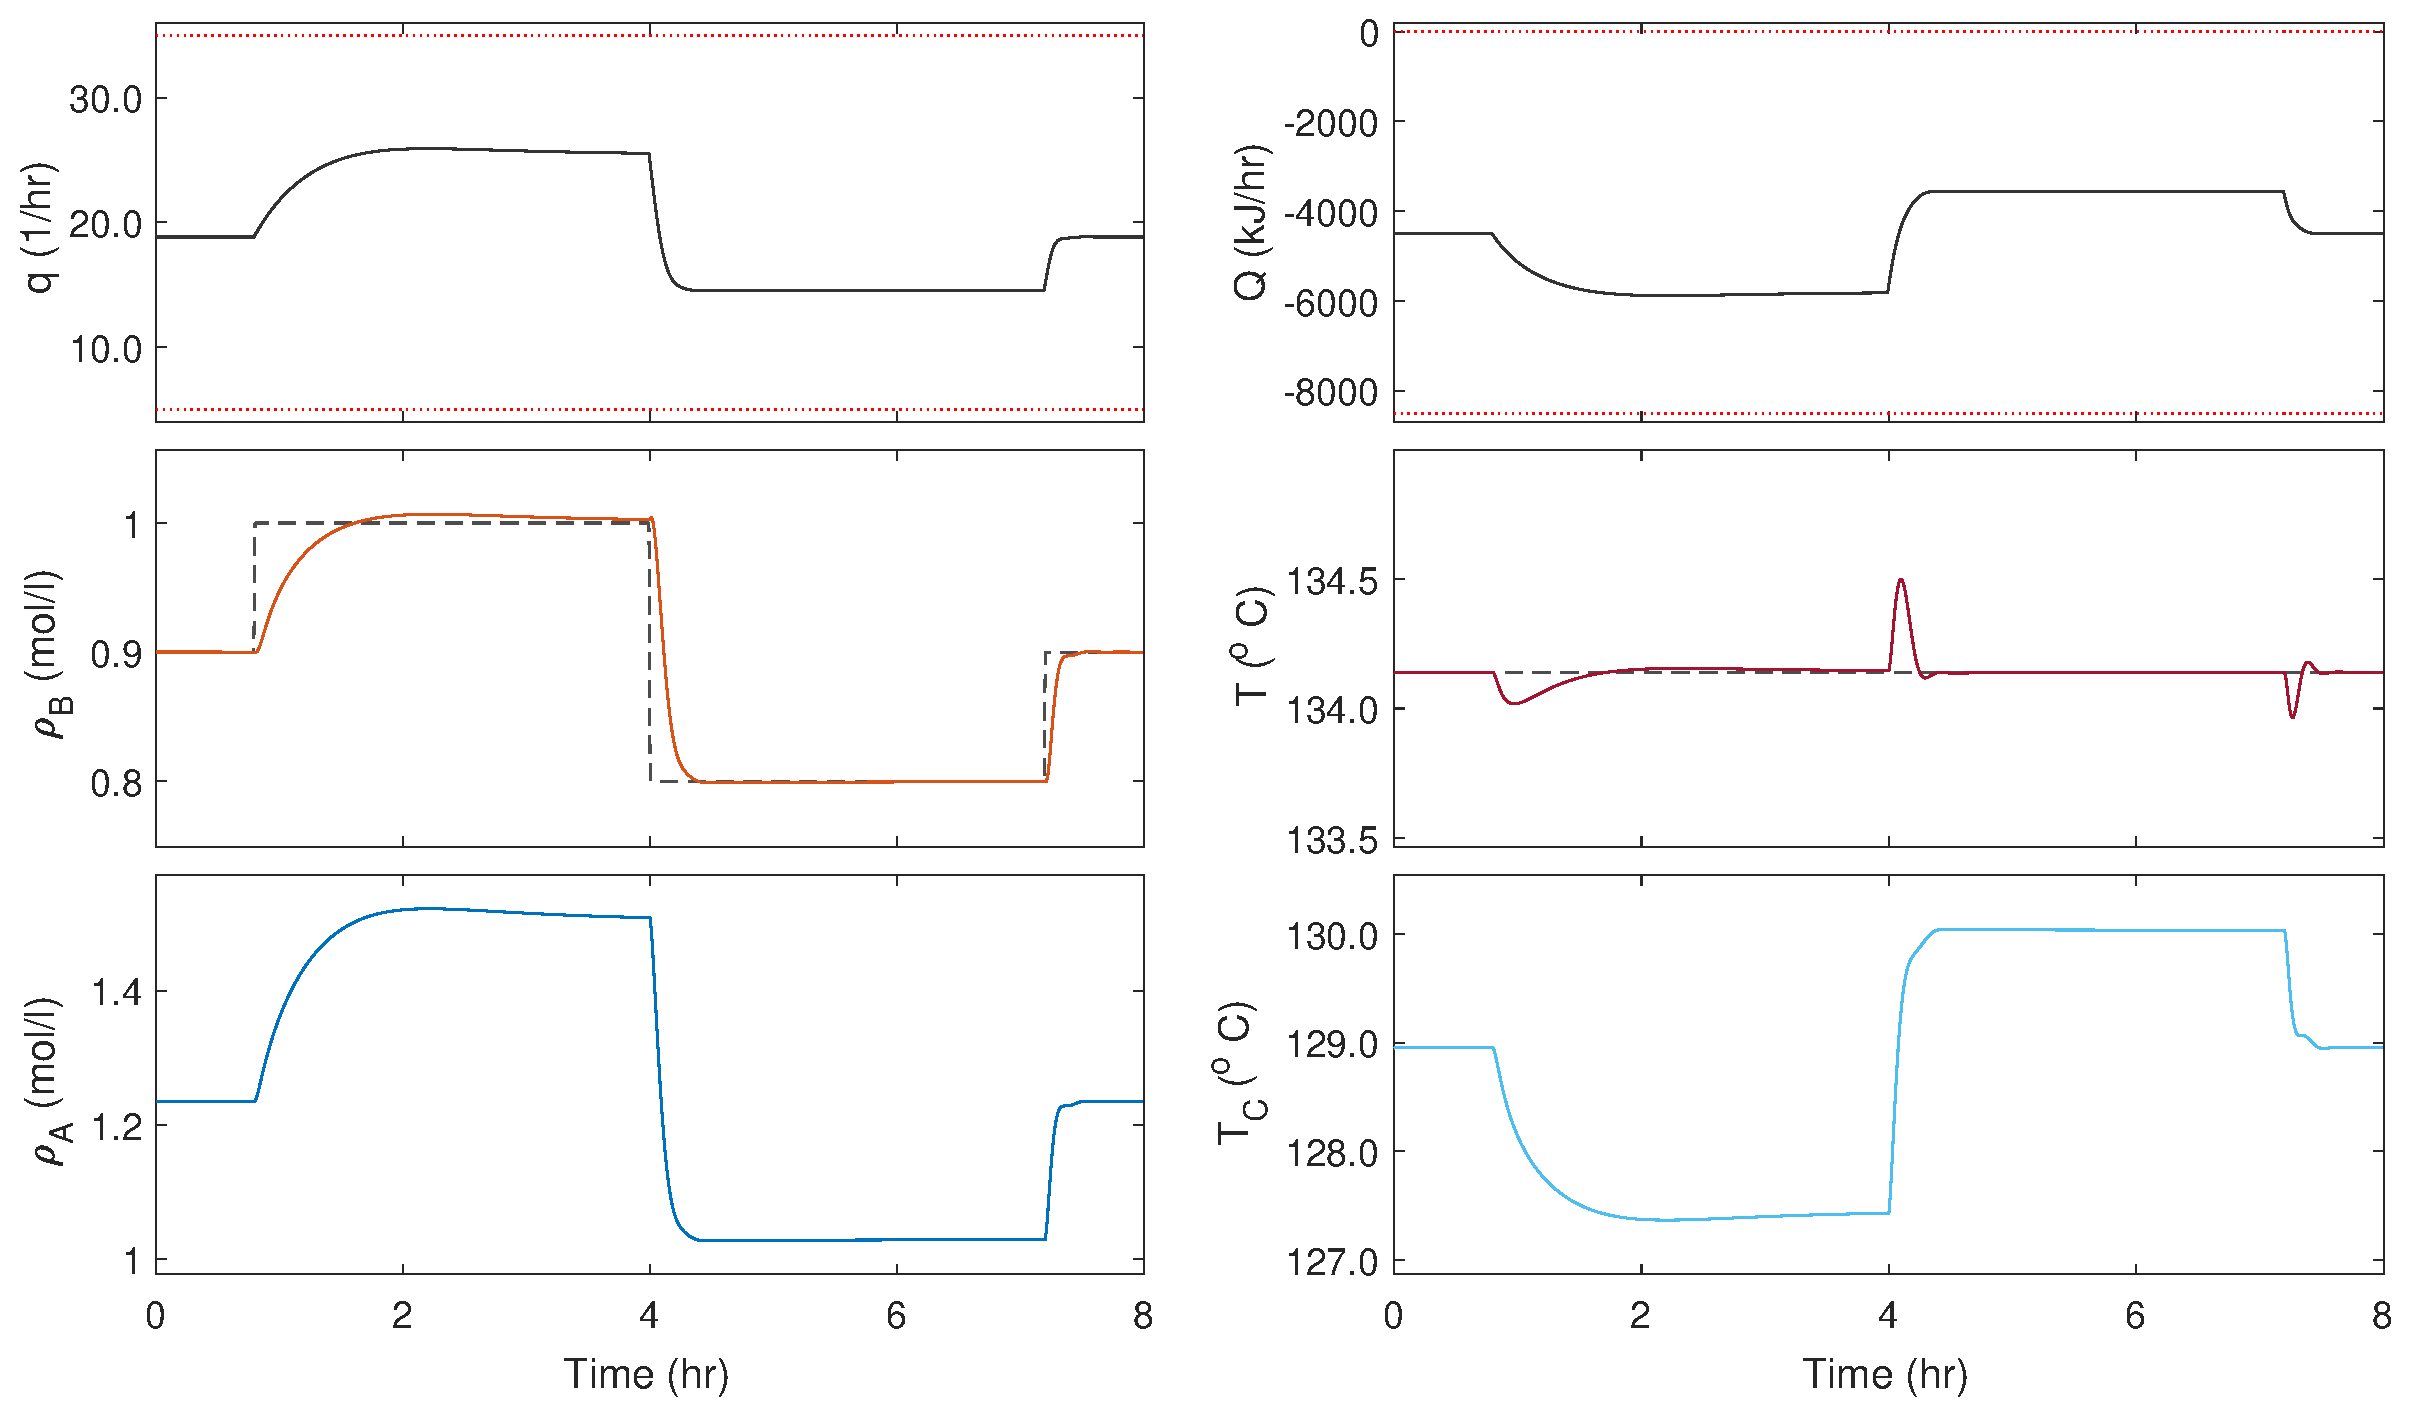
\includegraphics[width=\textwidth]{lqri01}
\end{figure}

\end{frame}

%-------------------------------------------------------
\begin{frame}[c]{Optimal Control}{Simulations}

\vskip0.25cm

\begin{figure}[h]
  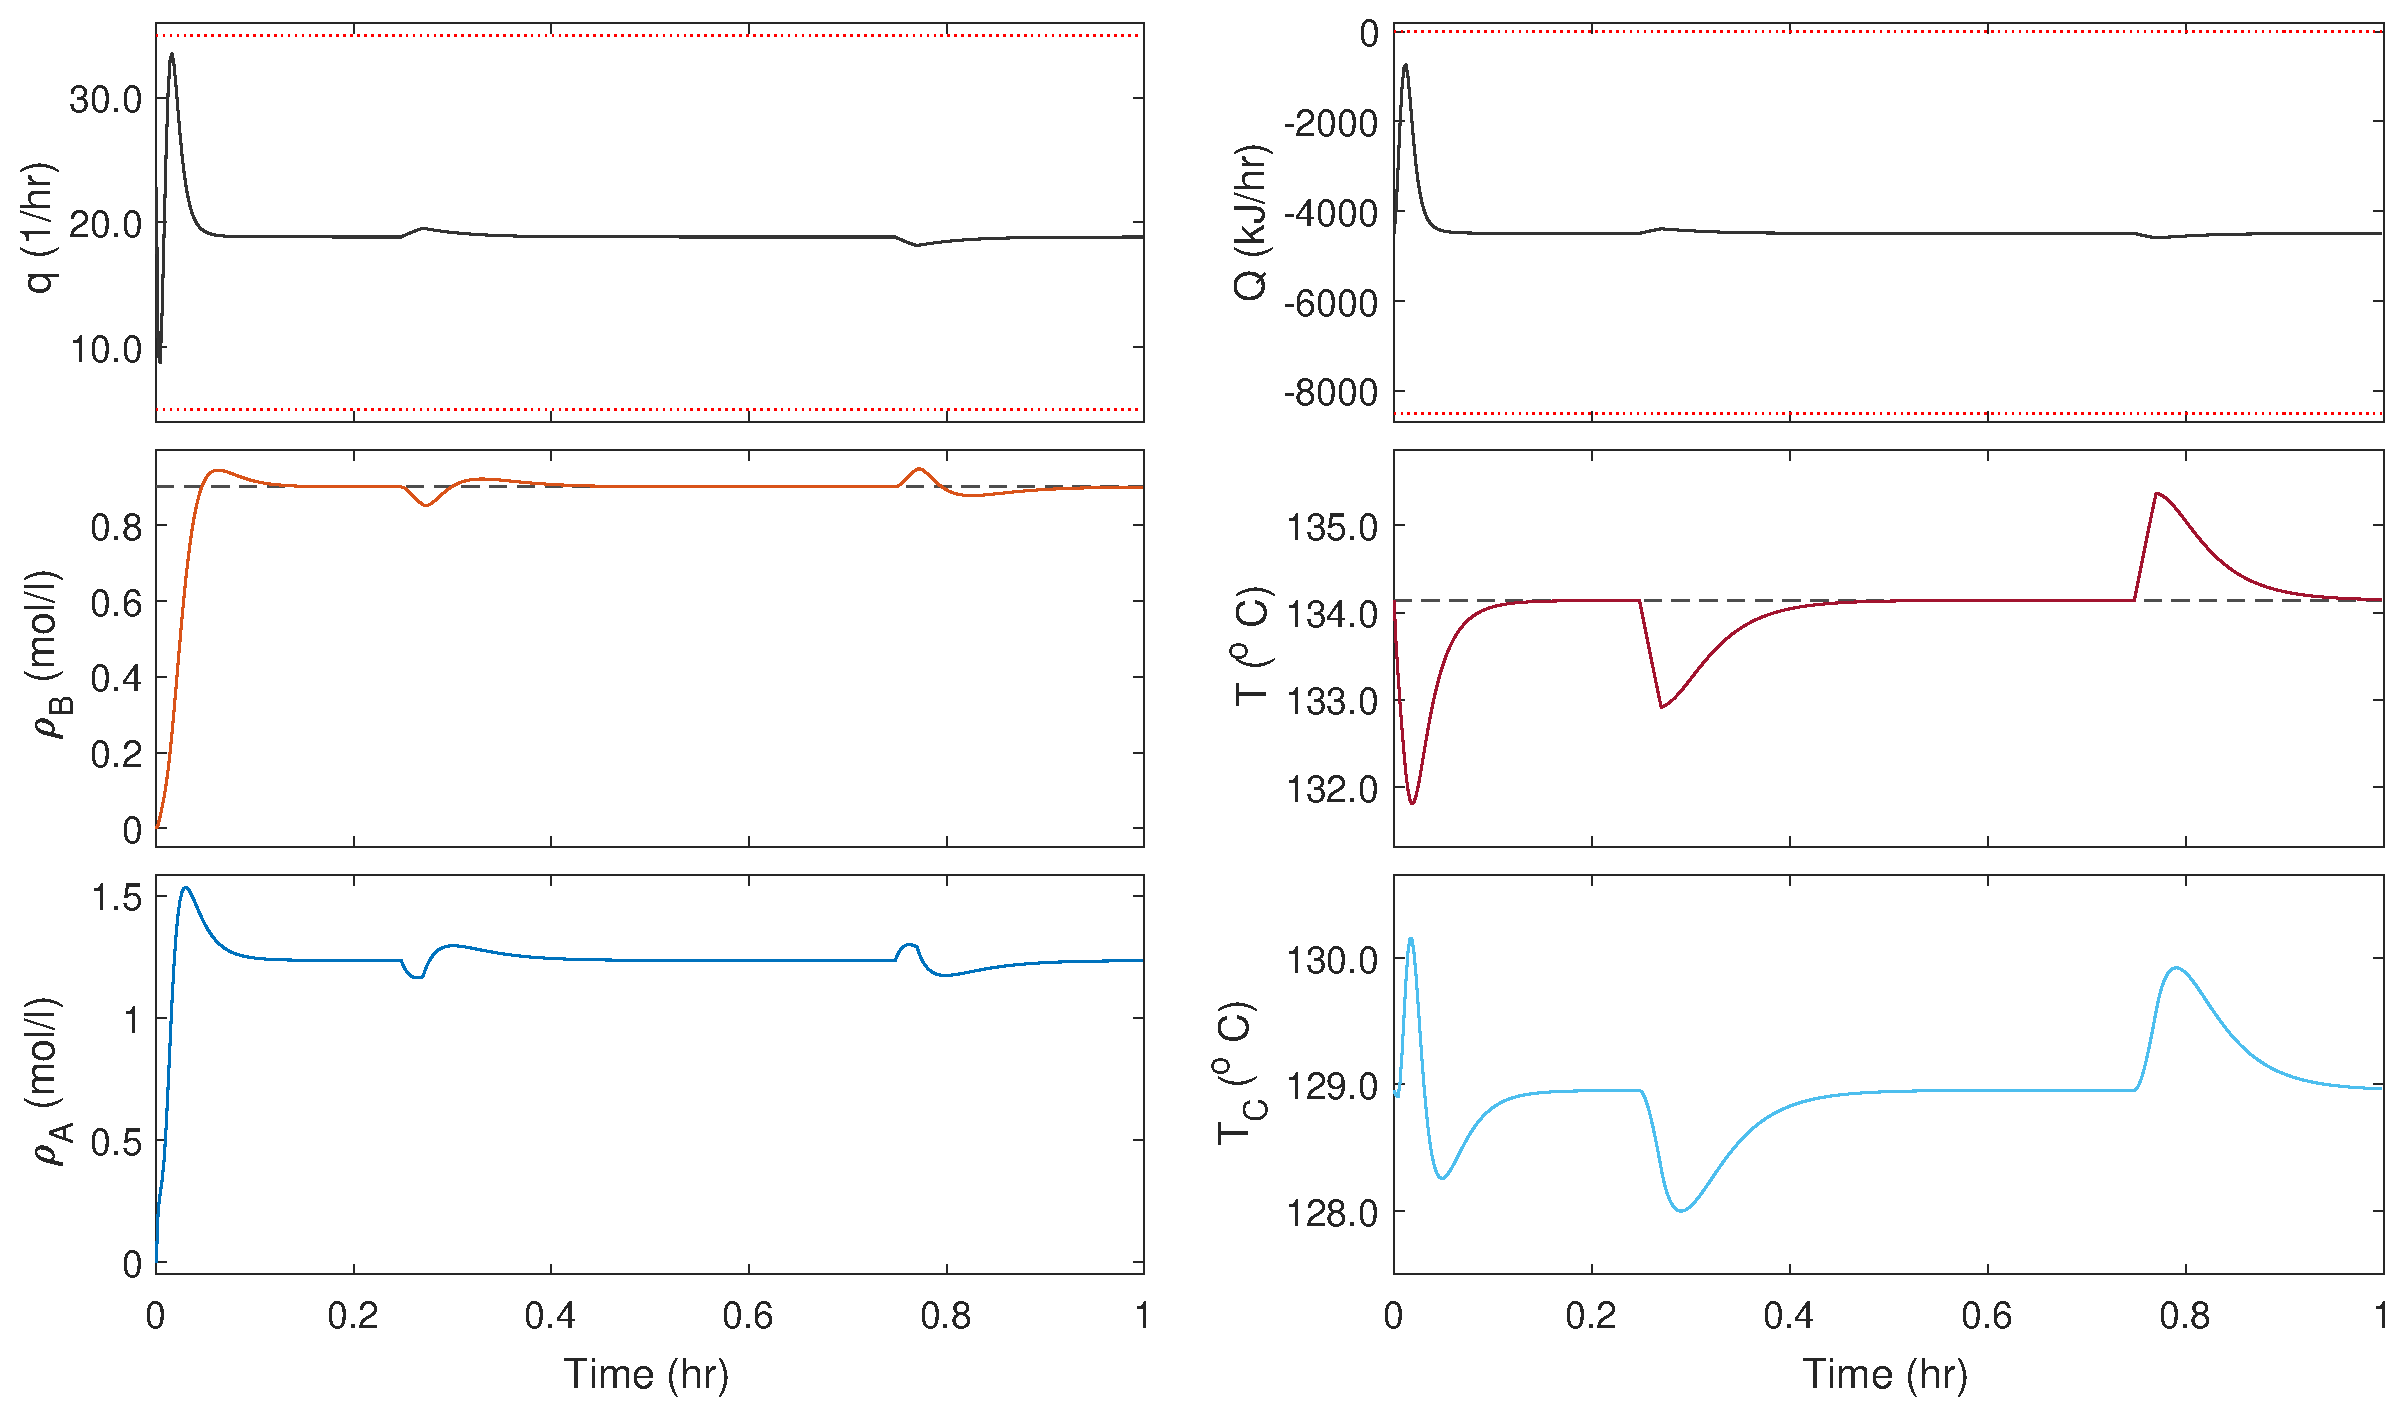
\includegraphics[width=\textwidth]{lqr02}
\end{figure}

\end{frame}

%-------------------------------------------------------
\begin{frame}[c]{Optimal Control}{Simulations}

\vskip0.25cm

\begin{figure}[h]
  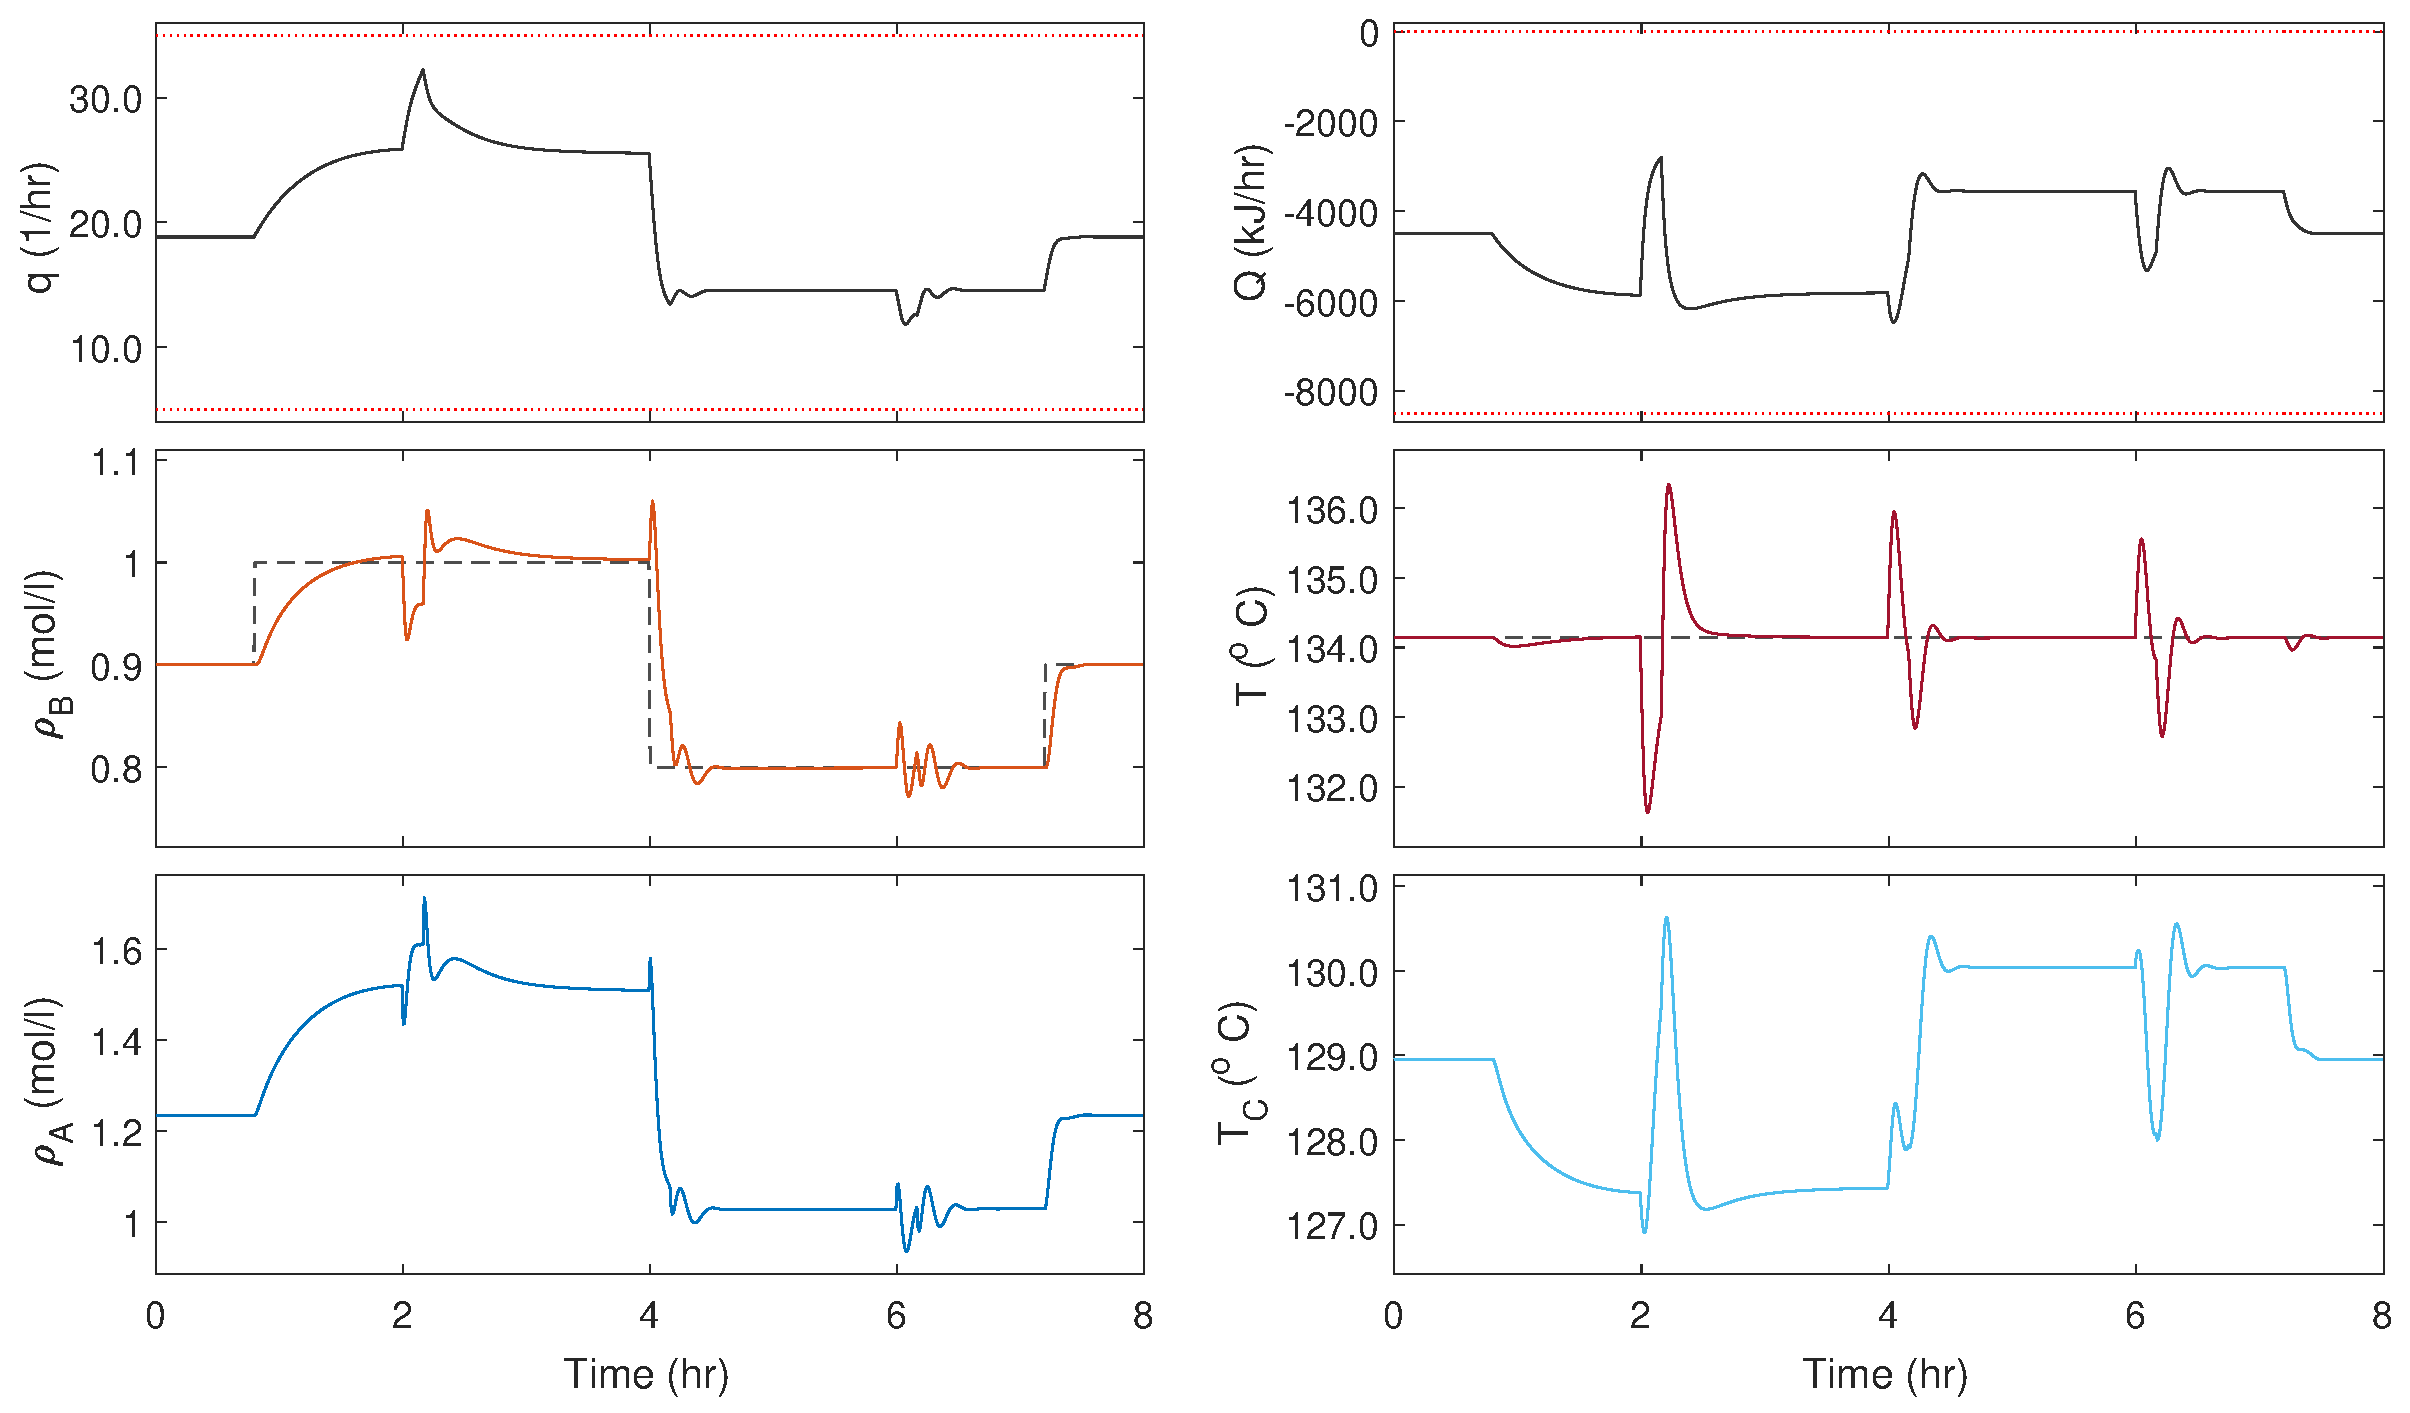
\includegraphics[width=\textwidth]{lqri02}
\end{figure}

\end{frame}

%-------------------------------------------------------
% SECTION - Optimal State Estimation
%-------------------------------------------------------
\section{Optimal State Estimation}
%-------------------------------------------------------
\subsection{Formulation}
%-------------------------------------------------------
\begin{frame}[t]{Optimal State Estimation}{Formulation}

\vskip0.1cm

\begin{itemize} \justifying
  \item<1-> We can \textbf{never} access real state of a physical system. \vskip0.2cm
  
  \begin{figure}[ht] \centering
      \resizebox{0.5\textwidth}{!}{
      \begin{tikzpicture}[auto, node distance=2cm,>=latex', scale=0.2]
          % We start by placing the blocks
          \node [input, name=input] {};
          \node [block, fill=glgBlue!10, right of=input, minimum width=10em, minimum height=5em, node distance=10em] (system) {Open-Loop System};
          \node [sum, right of=system, node distance=8em] (sensorSum) {};
          \node [text width=1em, above of=system, node distance=5em] (dW) {$\bm{w}$};
          \node [text width=1em, above of=sensorSum, node distance=5em] (dZ) {$\bm{z}$};
          \node [output, right of=sensorSum, node distance=3em] (output) {};
          
          % Once the nodes are placed, connecting them is easy.       
          \draw [draw,->] (input) -- node[pos=0.1] {${\color{signal1} \bm{u}}$}  (system);
          \draw [->] (system) -- node[pos=0.9] {$+$}  (sensorSum);
          \draw [->] (sensorSum) -- node[pos=0.9]{${\color{signal1} \bm{y}}$} (output);
          \draw [->] (dW) --  (system);
          \draw [->] (dZ) -- node[pos=0.9] {$+$} (sensorSum);
      \end{tikzpicture}}
  \end{figure} \vskip0.2cm

  \item<2|only@2> \textbf{Stochastic State-Space:} formulation that accounts for process and measurements uncertainty ($\bm{w}(t)$ and $\bm{v}(t)$, respectively).
  \begin{align*}
    \begin{cases}
        \hfill {\color{signal1} \dot{{\color{signal1} \bm{x}}}(t)} &= {\color{signal2} \bm{A}} {\color{signal1} {\color{signal1} \bm{x}}(t)} + {\color{signal2} \bm{B}} {\color{signal1} {\color{signal1} \bm{u}}(t)} + \bm{w}(t) \\
        \hfill {\color{signal1} {\color{signal1} \bm{y}}(t)} &= {\color{signal2} \bm{C}} {\color{signal1} {\color{signal1} \bm{x}}(t)} + \bm{v}(t)
    \end{cases}
    \end{align*}

  \item<3-> In probabilistic terms, we interpret the system as a Hidden Markov Model (HMM). \vskip0.2cm
  
  \begin{figure}[ht] \centering
      \resizebox{0.9\textwidth}{!}{
      \begin{tikzpicture}[auto, node distance=1.6cm,>=latex', scale=0.2]
          % Nodes
          \node [mcInput] (u0) {$u_0$};
          \node [mcCircleX, below of=u0] (x0) {$x_0$};
          \node [mcCircleY, below of=x0] (y0) {$y_0$};
          
          \node [mcInput, right of=u0] (u1) {$u_1$};
          \node [mcCircleX, below of=u1] (x1) {$x_1$};
          \node [mcCircleY, below of=x1] (y1) {$y_1$};
          
          \node [text width=2em, right of=x1] (cdots1) {$\cdots$};    
          
      \node [mcCircleX, right of=cdots1] (xi1) {$x_{k-1}$};     
          \node [mcInput, above of=xi1] (ui1) {$u_{k-1}$};
          \node [mcCircleY, below of=xi1] (yi1) {$y_{k-1}$};        
          
          \node [mcCircleX, right of=xi1] (xi2) {$x_{k}$};     
          \node [mcInput, above of=xi2] (ui2) {$u_{k}$};
          \node [mcCircleY, below of=xi2] (yi2) {$y_{k}$};
          
      \node [mcCircleX, right of=xi2] (xi3) {$x_{k+1}$};     
          \node [mcInput, above of=xi3] (ui3) {$u_{k+1}$};
          \node [mcCircleY, below of=xi3] (yi3) {$y_{k+1}$};        
          
          \node [text width=2em, right of=xi3] (cdots2) {$\cdots$};
          
          \node [mcCircleX, right of=cdots2] (xk) {$x_K$};
          \node [mcCircleY, below of=xk] (yk) {$y_K$};
          
          % Lines
          \draw [->,line width=.5mm] (u0) -- (x1);
          \draw [->,line width=.5mm] (u1) -- (cdots1);
          \draw [->,line width=.5mm] (ui1) -- (xi2);
          \draw [->,line width=.5mm] (ui2) -- (xi3);
          \draw [->,line width=.5mm] (ui3) -- (cdots2);
          
          \draw [->,line width=.5mm] (x0) -- (x1);
          \draw [->,line width=.5mm] (x1) -- (cdots1);
          \draw [->,line width=.5mm] (cdots1) -- (xi1);
          \draw [->,line width=.5mm] (xi1) -- (xi2);
          \draw [->,line width=.5mm] (xi2) -- (xi3);
          \draw [->,line width=.5mm] (xi3) -- (cdots2);
          \draw [->,line width=.5mm] (cdots2) -- (xk);
         
          \draw [->,line width=.5mm] (x0) -- (y0);
          \draw [->,line width=.5mm] (x1) -- (y1);
          \draw [->,line width=.5mm] (xi1) -- (yi1);
          \draw [->,line width=.5mm] (xi2) -- (yi2);
          \draw [->,line width=.5mm] (xi3) -- (yi3);
          \draw [->,line width=.5mm] (xk) -- (yk);
      \end{tikzpicture}}
\end{figure}

\end{itemize}

\end{frame}

%-------------------------------------------------------
\begin{frame}[t]{Optimal State Estimation}{Formulation}

\vskip0.25cm

\begin{varblock}[1\textwidth]{Closed-Loop Observer} 
    Given a system in State-Space with output signal ${\color{signal1} {\color{signal1} \bm{y}}(t)} : \mathbb{R} \rightarrow \mathbb{R}^p$ and an observer gain ${\color{signal4} \bm{L}} \in \mathbb{R}^{n \times p}$, the estimated state-vector ${\color{signal1} \hat{{\color{signal1} \bm{x}}}(t)}$ is represented by the system:
    \begin{equation*}
        {\color{signal1} \dot{\hat{{\color{signal1} \bm{x}}}}(t)} = {\color{signal2} \bm{A}} {\color{signal1} \hat{{\color{signal1} \bm{x}}}(t)} + {\color{signal2} \bm{B}} {\color{signal1} {\color{signal1} \bm{u}}(t)} + {\color{signal4} \bm{L}} \left( {\color{signal1} {\color{signal1} \bm{y}}(t)} - {\color{signal2} \bm{C}} {\color{signal1} \hat{{\color{signal1} \bm{x}}}(t)} \right)
    ,\end{equation*}
    
    \noindent or, equivalently:
    \begin{equation*}
        {\color{signal1} \dot{\hat{{\color{signal1} \bm{x}}}}(t)} = \left( {\color{signal2} \bm{A}} - {\color{signal4} \bm{L}} {\color{signal2} \bm{C}} \right) {\color{signal1} \hat{{\color{signal1} \bm{x}}}(t)} + {\color{signal2} \bm{B}} {\color{signal1} {\color{signal1} \bm{u}}(t)} + {\color{signal4} \bm{L}} {\color{signal1} {\color{signal1} \bm{y}}(t)}
    .\end{equation*} \vskip0.2cm
\end{varblock} \vskip0.2cm

\begin{itemize} \justifying
  \item<2-> The observer is operated in parallel to the actual system; \vskip0.2cm
  
  \item<3-> Consider a variable $\bm{e}(t) = {\color{signal1} {\color{signal1} \bm{x}}(t)} - {\color{signal1} \hat{{\color{signal1} \bm{x}}}(t)}$ such that:
  \begin{align*}
  \begin{split}
      \dot{\bm{e}} &= {\color{signal1} \bm{x}} - \hat{{\color{signal1} \bm{x}}} \\ 
          &= \left( {\color{signal2} \bm{A}} - {\color{signal4} \bm{L}} {\color{signal2} \bm{C}} \right) \left( {\color{signal1} \bm{x}} - \hat{{\color{signal1} \bm{x}}} \right) \\
          &= \left( {\color{signal2} \bm{A}} - {\color{signal4} \bm{L}} {\color{signal2} \bm{C}} \right) \bm{e}
  \end{split}
  \end{align*} \vskip0.2cm
  
  \item<4-> \textbf{Control-Estimator Duality:} the design of ${\color{signal4} \bm{L}}$ follows the same design procedure of ${\color{signal4} \bm{K}}$.
\end{itemize}

\end{frame}

%-------------------------------------------------------
\subsection{Kalman Filter and LQG Controllers}
%-------------------------------------------------------
\begin{frame}[t]{Optimal State Estimation}{Kalman Filter and Linear Quadratic Gaussian (LQG)}

\vskip0.25cm

\begin{varblock}[1\linewidth]{Kalman-Bucy Optimal Filter} \justifying
  Consider a model subject to a additive process noise variable $\bm{w}(t) \sim \mathcal{N}(\bm{0}, {\color{signal3} \bm{Q}}_{kf})$ and a measurement noise variable $\bm{v}(t) \sim \mathcal{N}(\bm{0}, {\color{signal3} \bm{R}}_{kf})$. In this case, for an estimated state ${\color{signal1} \hat{{\color{signal1} \bm{x}}}(t)}$ at time $t$, the error covariance:
    \begin{equation*}
        \bm{J}({\color{signal1} \bm{x}}, \hat{{\color{signal1} \bm{x}}}, t) = \mathbb{E}\left\{ [{\color{signal1} {\color{signal1} \bm{x}}(t)} - {\color{signal1} \hat{{\color{signal1} \bm{x}}}(t)}][{\color{signal1} {\color{signal1} \bm{x}}(t)} - {\color{signal1} \hat{{\color{signal1} \bm{x}}}(t)}]^T \right\}
    \end{equation*}
    
    \noindent is minimized by a ${\color{signal1} \hat{{\color{signal1} \bm{x}}}(t)}$ obtained through the system:
    \begin{equation*}
        {\color{signal1} \dot{\hat{{\color{signal1} \bm{x}}}}(t)} = {\color{signal2} \bm{A}} {\color{signal1} \hat{{\color{signal1} \bm{x}}}(t)} + {\color{signal2} \bm{B}} {\color{signal1} {\color{signal1} \bm{u}}(t)} + {\color{signal4} \bm{K}}_{e}(t) \left( {\color{signal1} {\color{signal1} \bm{y}}(t)} - {\color{signal2} \bm{C}} {\color{signal1} \hat{{\color{signal1} \bm{x}}}(t)} \right)
    ,\end{equation*}
    
    \noindent where ${\color{signal4} \bm{K}}_e(t) = {\color{signal3} \bm{P}}_e(t){\color{signal2} \bm{C}}{\color{signal3} \bm{R}}^{-1}$, being ${\color{signal3} \bm{P}}_e(t)$ the solution of the Riccati differential matrix equation:
    \begin{equation*}
        \dot{{\color{signal3} \bm{P}}_e}(t) = {\color{signal2} \bm{A}} {\color{signal3} \bm{P}}_e(t) + {\color{signal3} \bm{P}}_e(t) {\color{signal2} \bm{A}}^T - {\color{signal3} \bm{P}}_e(t){\color{signal2} \bm{C}}^T{\color{signal3} \bm{R}}_{kf}^{-1} {\color{signal2} \bm{C}} {\color{signal3} \bm{P}}_e(t) + {\color{signal3} \bm{Q}}_{kf}
    ,\end{equation*}
    
    \noindent with initial condition ${\color{signal3} \bm{P}}_e(t_0) = \mathbb{E} \left\{ [{\color{signal1} \bm{x}}(t_0) - \bar{{\color{signal1} \bm{x}}}(t_0)][{\color{signal1} \bm{x}}(t_0) - \bar{{\color{signal1} \bm{x}}}(t_0)]^T \right\}$ for $t_0 > -\infty$.
\end{varblock}

\end{frame}

%-------------------------------------------------------
\begin{frame}[t]{Optimal State Estimation}{Formulation}

\vskip0.25cm

\begin{varblock}[1\textwidth]{The Separation Principle} 
    Given a system in State-Space with a Luenberger observer of gain ${\color{signal4} \bm{L}}$ and state-feedback controller of gain ${\color{signal4} \bm{K}}$, the closed-loop eigenvalues contributions of $({\color{signal2} \bm{A}} - {\color{signal2} \bm{B}}{\color{signal4} \bm{K}})$ are independent from those of $({\color{signal2} \bm{A}} - {\color{signal4} \bm{L}}{\color{signal2} \bm{C}})$.
\end{varblock} \vskip0.3cm

\begin{itemize}
  \item<1-> It can be shown that the closed-loop dynamics of the system and the error reduces to:
  \begin{equation*}
    \begin{bmatrix} \dot{{\color{signal1} \bm{x}}} \\ \dot{\bm{e}}    \end{bmatrix}
    =
    \begin{bmatrix}
        {\color{signal2} \bm{A}} - {\color{signal2} \bm{B}} {\color{signal4} \bm{K}} & - {\color{signal2} \bm{B}} {\color{signal4} \bm{K}} \\
        \bm{0} & {\color{signal2} \bm{A}} - {\color{signal4} \bm{L}} {\color{signal2} \bm{C}}
    \end{bmatrix} \begin{bmatrix} {\color{signal1} \bm{x}} \\ \bm{e} \end{bmatrix}
    +
    \begin{bmatrix} {\color{signal2} \bm{B}} \\ \bm{0} \end{bmatrix} {\color{signal1} \bm{r}}
  \end{equation*} \vskip0.2cm
  
  \item<2-> The eigenvalues of the augmented system is the direct contribution of  the eigenvalues of $({\color{signal2} \bm{A}}- {\color{signal2} \bm{B}}{\color{signal4} \bm{K}})$ and $({\color{signal2} \bm{A}}- {\color{signal4} \bm{L}}{\color{signal2} \bm{C}})$. \vskip0.2cm
  
  \item<3-> \textbf{Direct Result:} the controller and the estimator can be designed separately, and they are \textit{dual problems}. 
\end{itemize}

\end{frame}


%-------------------------------------------------------
\begin{frame}[t]{Optimal State Estimation}{Kalman Filter and Linear Quadratic Gaussian (LQG)}

\vskip0.15cm

\begin{varblock}[1\linewidth]{Linear Quadratic Gaussian (LQG) Controller}
  Consider a stochastic system in State-Space representation:
  \begin{align*}
    \begin{cases}
        \hfill {\color{signal1} \dot{{\color{signal1} \bm{x}}}(t)} &= {\color{signal2} \bm{A}} {\color{signal1} {\color{signal1} \bm{x}}(t)} + {\color{signal2} \bm{B}} {\color{signal1} {\color{signal1} \bm{u}}(t)} + \bm{w}(t) \\
        \hfill {\color{signal1} {\color{signal1} \bm{y}}(t)} &= {\color{signal2} \bm{C}} {\color{signal1} {\color{signal1} \bm{x}}(t)} + \bm{v}(t)
    \end{cases}
    ,\end{align*}
    
     \noindent whose state-vector is determined by a Kalman-Bucy filter and whose input signal is calculated by a finite-horizon LQR. The Linear Quadratic Gaussian (LQG) is defined as:
    \begin{align*} 
        {\color{signal1} \dot{\hat{{\color{signal1} \bm{x}}}}(t)} = \left[{\color{signal2} \bm{A}} - {\color{signal4} \bm{K}}_e(t) {\color{signal2} \bm{C}} - {\color{signal2} \bm{B}} {\color{signal4} \bm{K}}(t) \right] {\color{signal1} \hat{{\color{signal1} \bm{x}}}(t)} + {\color{signal4} \bm{K}}_e(t) {\color{signal1} {\color{signal1} \bm{y}}(t)} 
    ,\end{align*}
    
    \noindent where ${\color{signal4} \bm{K}}(t) = {\color{signal3} \bm{R}}^{-1}{\color{signal2} \bm{B}}^T {\color{signal3} \bm{P}}(t)$ and ${\color{signal4} \bm{K}}_e(t) = {\color{signal3} \bm{P}}_e(t) {\color{signal2} \bm{C}} {\color{signal3} \bm{R}}^{-1}$ are, respectively, the LQR and Kalman-Bucy gains for matrices ${\color{signal3} \bm{P}}(t)$ and ${\color{signal3} \bm{P}}_e(t)$ that solve the Riccati differential equations:
    \begin{align*}
    \begin{cases}
        -\dot{{\color{signal3} \bm{P}}}(t) = {\color{signal2} \bm{A}}^T {\color{signal3} \bm{P}}(t) + {\color{signal3} \bm{P}}(t) {\color{signal2} \bm{A}} - {\color{signal3} \bm{P}}(t) {\color{signal2} \bm{B}} {\color{signal3} \bm{R}}^{-1} {\color{signal2} \bm{B}}^T {\color{signal3} \bm{P}}(t) + {\color{signal3} \bm{Q}} \\
        \phantom{-} \dot{{\color{signal3} \bm{P}}_e}(t) = {\color{signal2} \bm{A}} {\color{signal3} \bm{P}}_e(t) + {\color{signal3} \bm{P}}_e(t) {\color{signal2} \bm{A}}^T - {\color{signal3} \bm{P}}_e(t){\color{signal2} \bm{C}}^T{\color{signal3} \bm{R}}_{kf}^{-1} {\color{signal2} \bm{C}} {\color{signal3} \bm{P}}_e(t) + {\color{signal3} \bm{Q}}_{kf}
    \end{cases}
    \end{align*}
    
    \noindent for boundary conditions ${\color{signal3} \bm{P}}(T) = {\color{signal3} \bm{Q}}_f$ and ${\color{signal3} \bm{P}}_e(t_0) = \mathbb{E} \left\{ [{\color{signal1} \bm{x}}(t_0) - \bar{{\color{signal1} \bm{x}}}(t_0)][{\color{signal1} \bm{x}}(t_0) - \bar{{\color{signal1} \bm{x}}}(t_0)]^T \right\}$, respectively.
\end{varblock}

\end{frame}

%-------------------------------------------------------
\begin{frame}[c]{Optimal State Estimation}{Kalman Filter and Linear Quadratic Gaussian (LQG)}

\vskip0.25cm

\begin{figure}[ht]
    \centering
    \resizebox{0.95\textwidth}{!}{
    \begin{tikzpicture}[auto, node distance=1.75cm,>=latex']
        % We start by placing the blocks
        \node [input, name=input] {};
        \node [sum, right of=input, node distance=3em] (intFbckSum) {};
        \node [block, right of=intFbckSum, node distance=4em] (integralAction) {$\int$};
        \node [block, right of=integralAction, node distance=6em] (intActGain) {${\color{signal4} \bm{K}}_a$};
        \node [sum, right of=intActGain, node distance=4.5em] (fbckSum) {};

        \node [block, fill=glgBlue!20, minimum height=4em, right of=fbckSum, node distance=14em] (openloopSystem) {Open-Loop System};    
        \node [output, right of=outputMatrix, node distance=10em] (output) {};
        
        \node [block, below of=openloopSystem, node distance=14em] (integralLU) {$\int$};     
        \node [sum, left of=integralLU, node distance=4em] (stateSumLU) {};             
        \node [block, left of=stateSumLU, node distance=4em] (inputMatrixLU) {${\color{signal2} \bm{B}}$};
        \node [block, right of=integralLU, node distance=8em] (outputMatrixLU) {${\color{signal2} \bm{C}}$};
        \node [block, below of=integralLU] (stateMatrixLU) {${\color{signal2} \bm{A}}$};
        \node [block, above of=integralLU] (kalmanGain) {${\color{signal4} \bm{K}}_e$};       
        
        \draw [->] (openloopSystem) -- node[name=bk3,pos=0.5]{} node[name=bk5,pos=0.75]{} node[pos=0.9]{${\color{signal1} \bm{y}}$} (output);
        \node [sum, anchor=base] (fbckOutput) at (bk3.base |- kalmanGain) {};
        
        \node [block, below of=stateSumLU, node distance=12em, label={below:LQR Controller}] (fbckGain) {${\color{signal4} \bm{K}}$};     
        
        
        \begin{scope}[on background layer]
            \node [fit=(integralAction) (intActGain), fill= glgGreen!10, rounded corners, inner sep=.4cm, label={[xshift=4.3em, glgGreen!90]above left:Integral Action}] {};
        \end{scope} 
        
        \begin{scope}[on background layer]
            \node [fit=(inputMatrixLU) (kalmanGain) (stateMatrixLU) (fbckOutput), fill= glgRed!10, rounded corners, inner sep=.4cm, label={[xshift=5.75em, glgRed!90]above left:Kalman-Bucy Filter}] {};
        \end{scope} 
        
        % Once the nodes are placed, connecting them is easy.       
        \draw [draw,->] (input) -- node[pos=0.1] {${\color{signal1} \bm{r}}$} node[pos=0.8] {$+$}  (intFbckSum);
        \draw [->] (intFbckSum) -- (integralAction);
        \draw [->] (integralAction) -- node[pos=0.5]{${\color{signal1} \bm{x}}_a$} (intActGain);
        \draw [->] (intActGain) -- node[pos=0.8]{$-$} (fbckSum);        
        \draw [->] (fbckSum) -- node[pos=0.2]{${\color{signal1} \bm{u}}$} node[name=bku1, pos=0.2]{} (openloopSystem);
        

        \draw [->] (fbckGain) -| node[pos=0.98]{$-$} (fbckSum);
        \draw [->] (bk5) |- ++(0, -30em) -| node[pos=0.98]{$-$} (intFbckSum);
        
        
        \draw [->] (bku1) |- (inputMatrixLU);
        \draw [->] (inputMatrixLU) -- node[pos=0.8]{$+$} (stateSumLU);
        \draw [->] (stateSumLU) -- node[pos=0.5]{$\dot{\hat{{\color{signal1} \bm{x}}}}$} (integralLU);
        \draw [->] (integralLU) -- node[name=bk4,pos=0.5]{} node[pos=0.5]{$\hat{{\color{signal1} \bm{x}}}$} (outputMatrixLU);
        \draw [->] (outputMatrixLU) -| node[pos=0.95]{$-$} (fbckOutput);
        \draw [->] (bk4) |- (stateMatrixLU);
        \draw [->] (fbckOutput) -- (kalmanGain);
        \draw [->] (stateMatrixLU) -| node[pos=0.95]{$+$} (stateSumLU);
        \draw [->] (kalmanGain) -| node[pos=0.95]{$+$} (stateSumLU);
        \draw [->] (bk3) -- node[pos=0.95]{$+$} (fbckOutput);
        
        \draw [->] (bk4) |- (fbckGain);
    \end{tikzpicture} 
    }
\end{figure}

\end{frame}

%-------------------------------------------------------
\subsection{Simulations}
%-------------------------------------------------------
\begin{frame}[c]{Optimal Control}{Simulations}

\vskip0.25cm

\begin{figure}[h]
  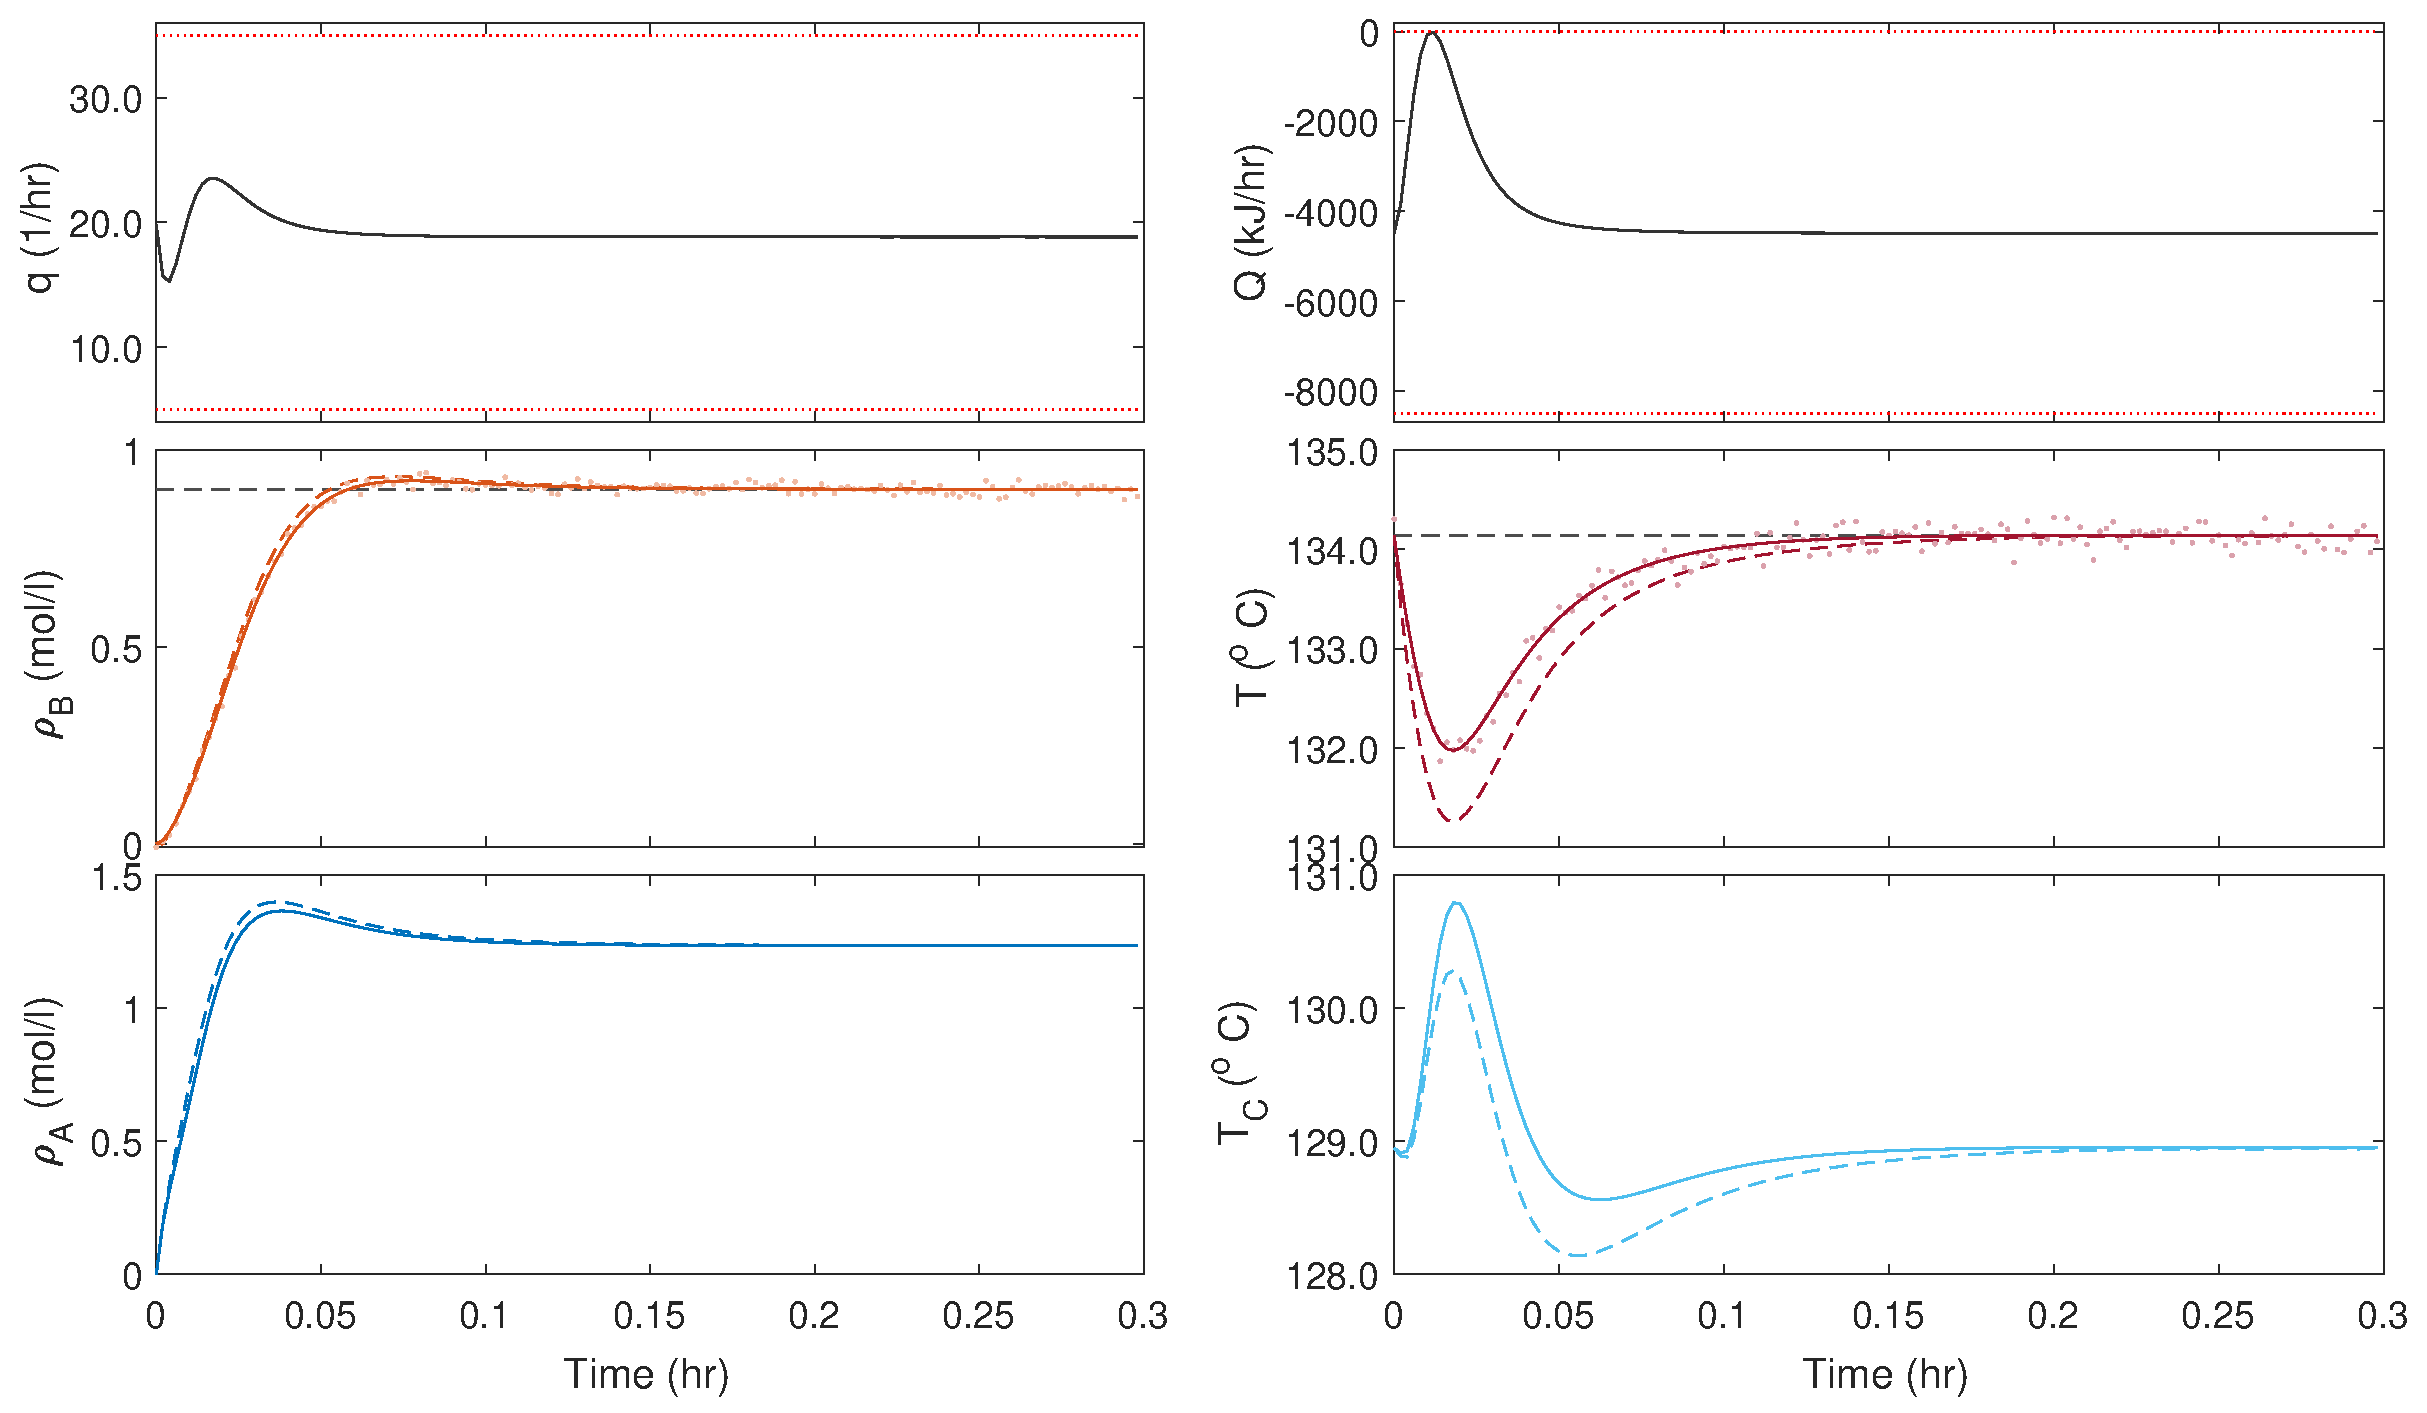
\includegraphics[width=\textwidth]{lqg01}
\end{figure}

\end{frame}

%-------------------------------------------------------
\begin{frame}[c]{Optimal Control}{Simulations}

\vskip0.25cm

\begin{figure}[h]
  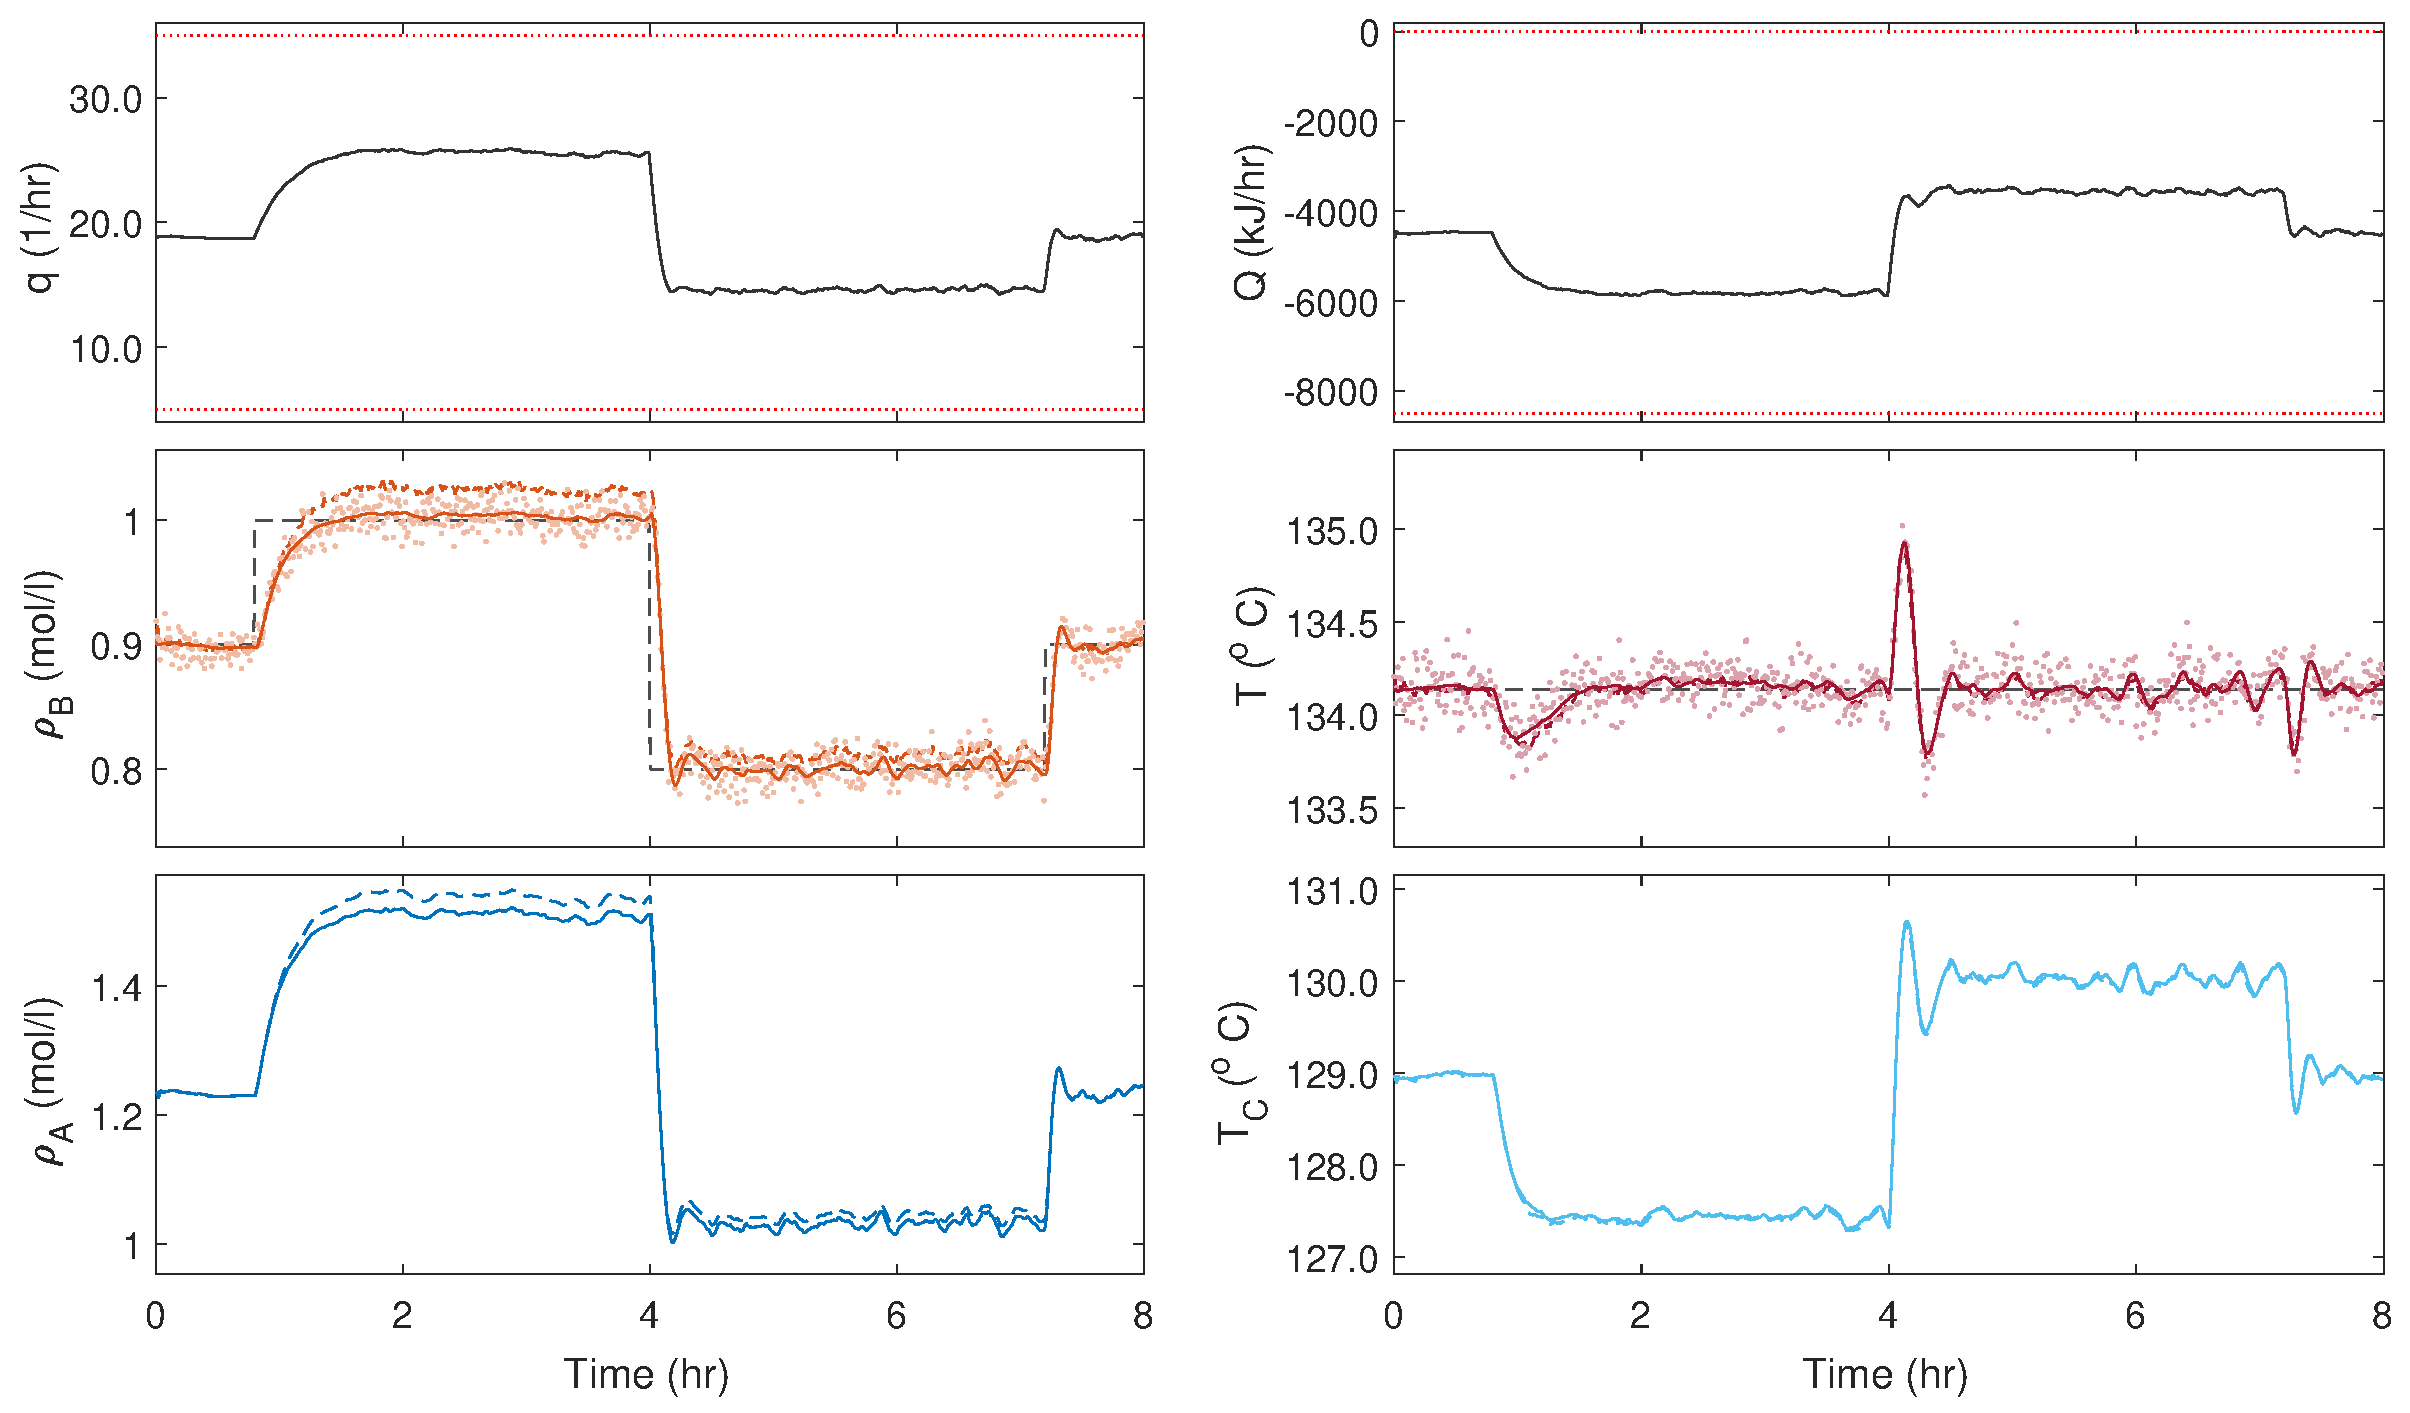
\includegraphics[width=\textwidth]{lqgi01}
\end{figure}

\end{frame}

%-------------------------------------------------------
\begin{frame}[c]{Optimal Control}{Simulations}

\vskip0.25cm

\begin{figure}[h]
  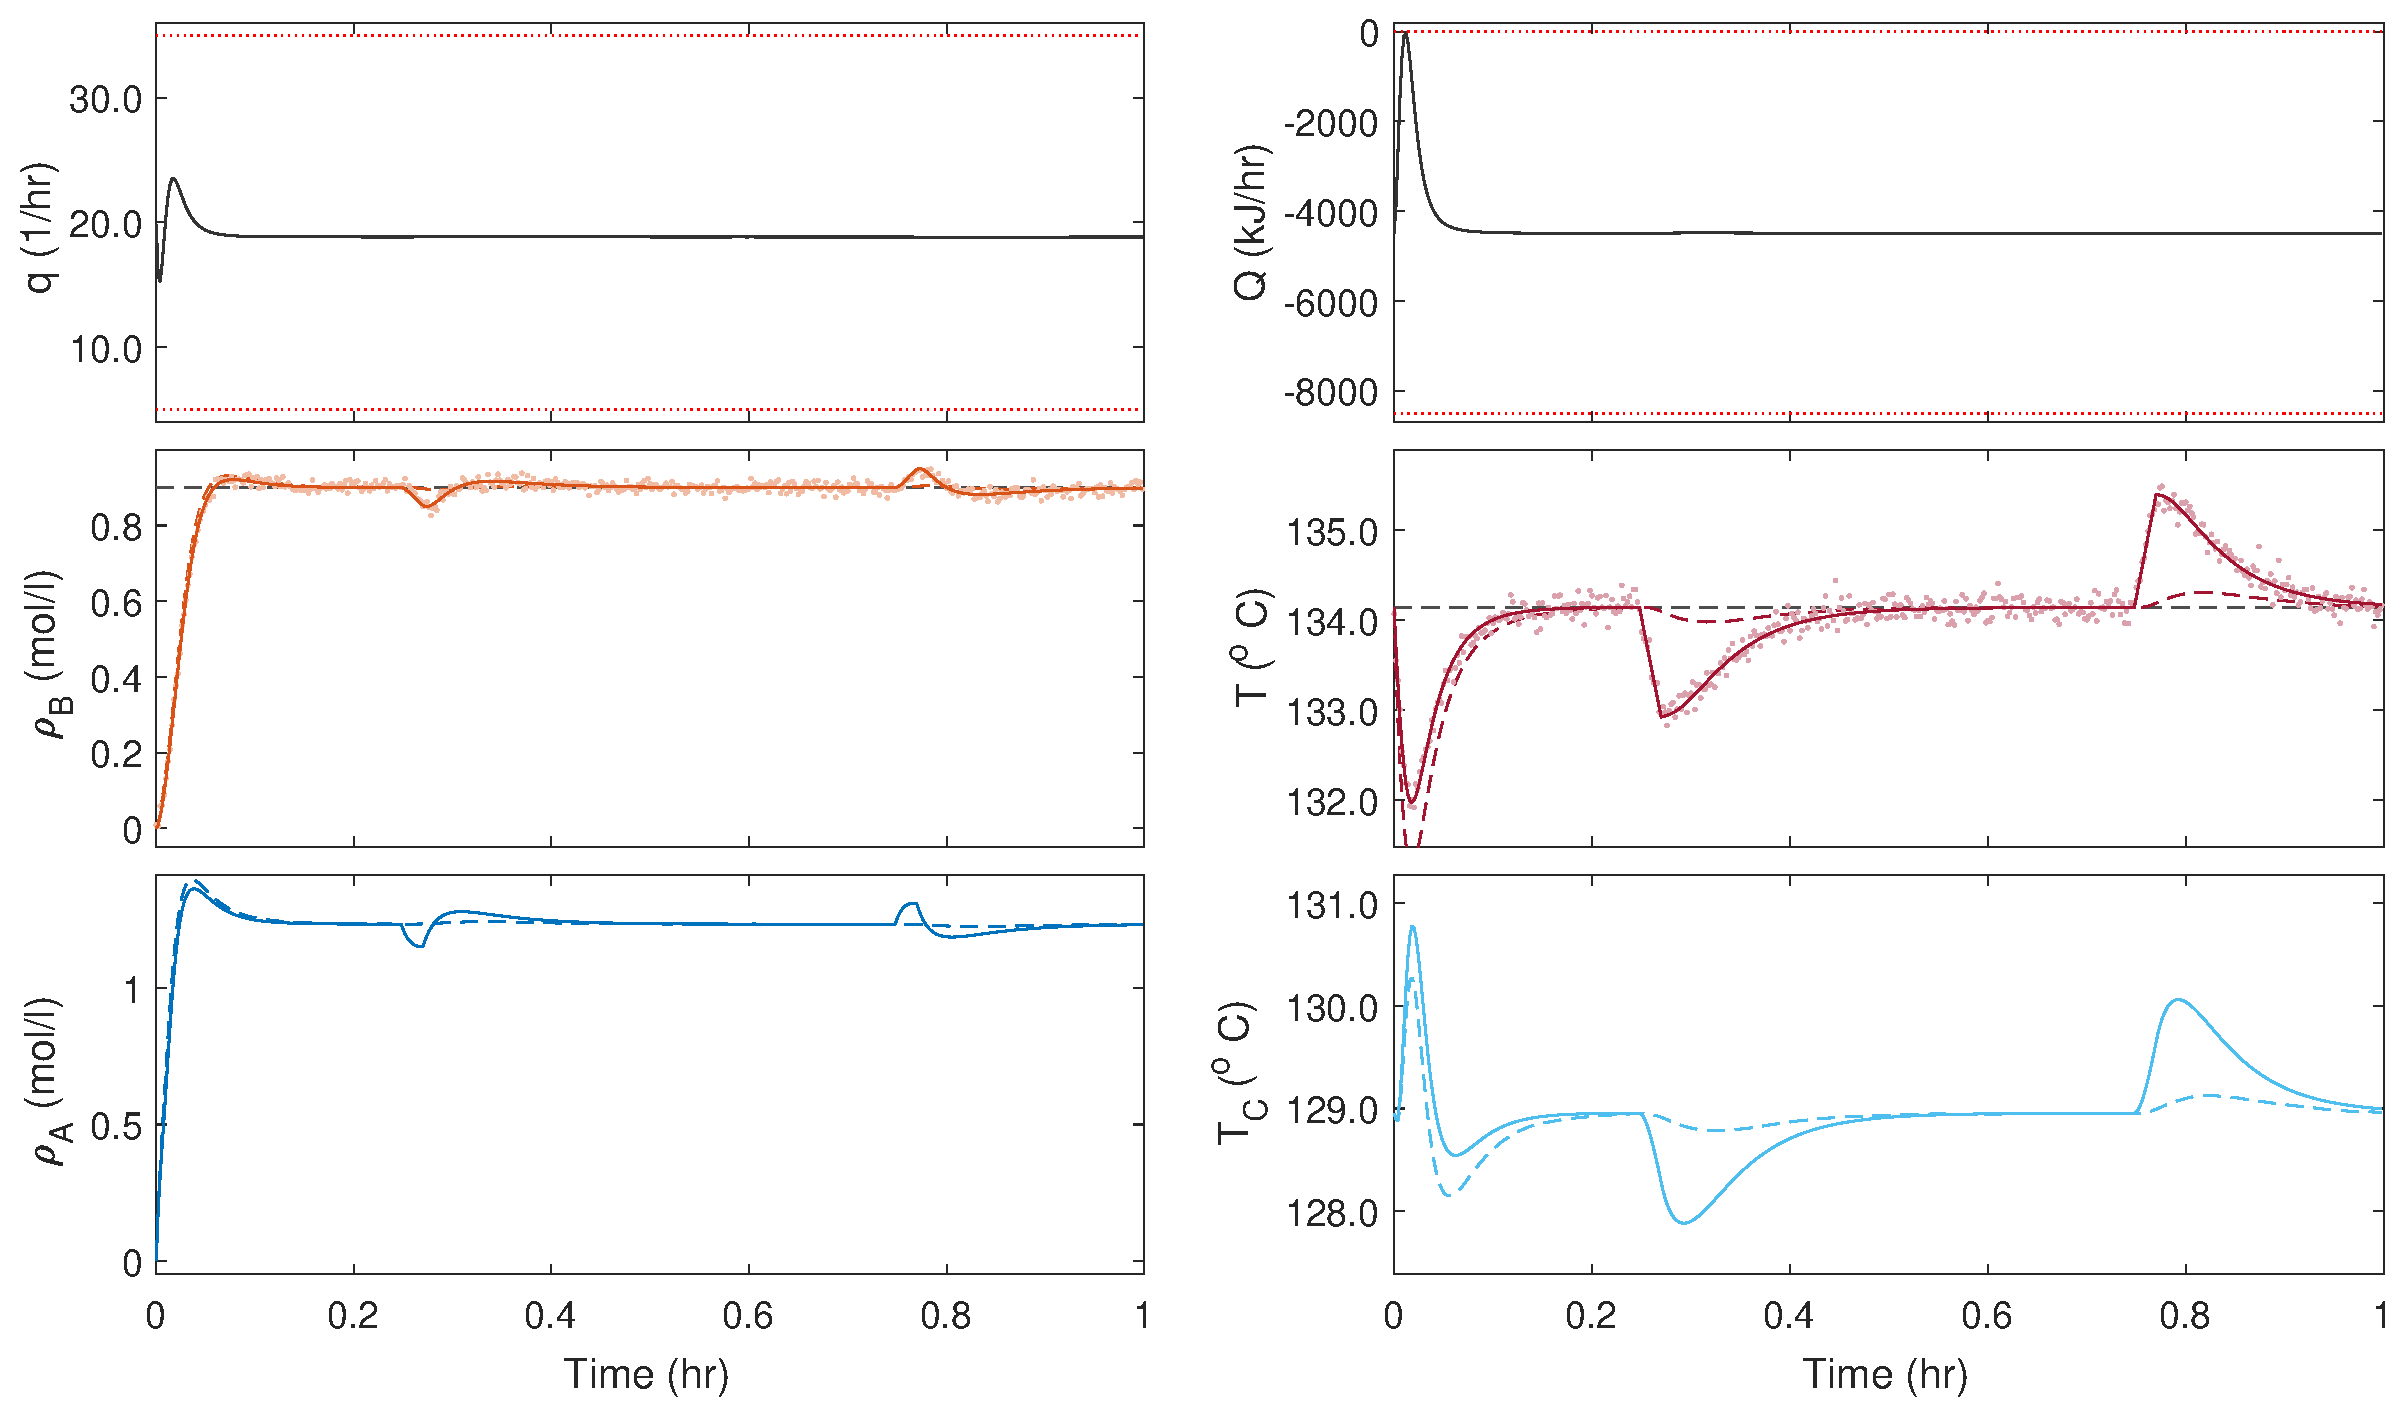
\includegraphics[width=\textwidth]{lqg02}
\end{figure}

\end{frame}

%-------------------------------------------------------
\begin{frame}[c]{Optimal Control}{Simulations}

\vskip0.25cm

\begin{figure}[h]
  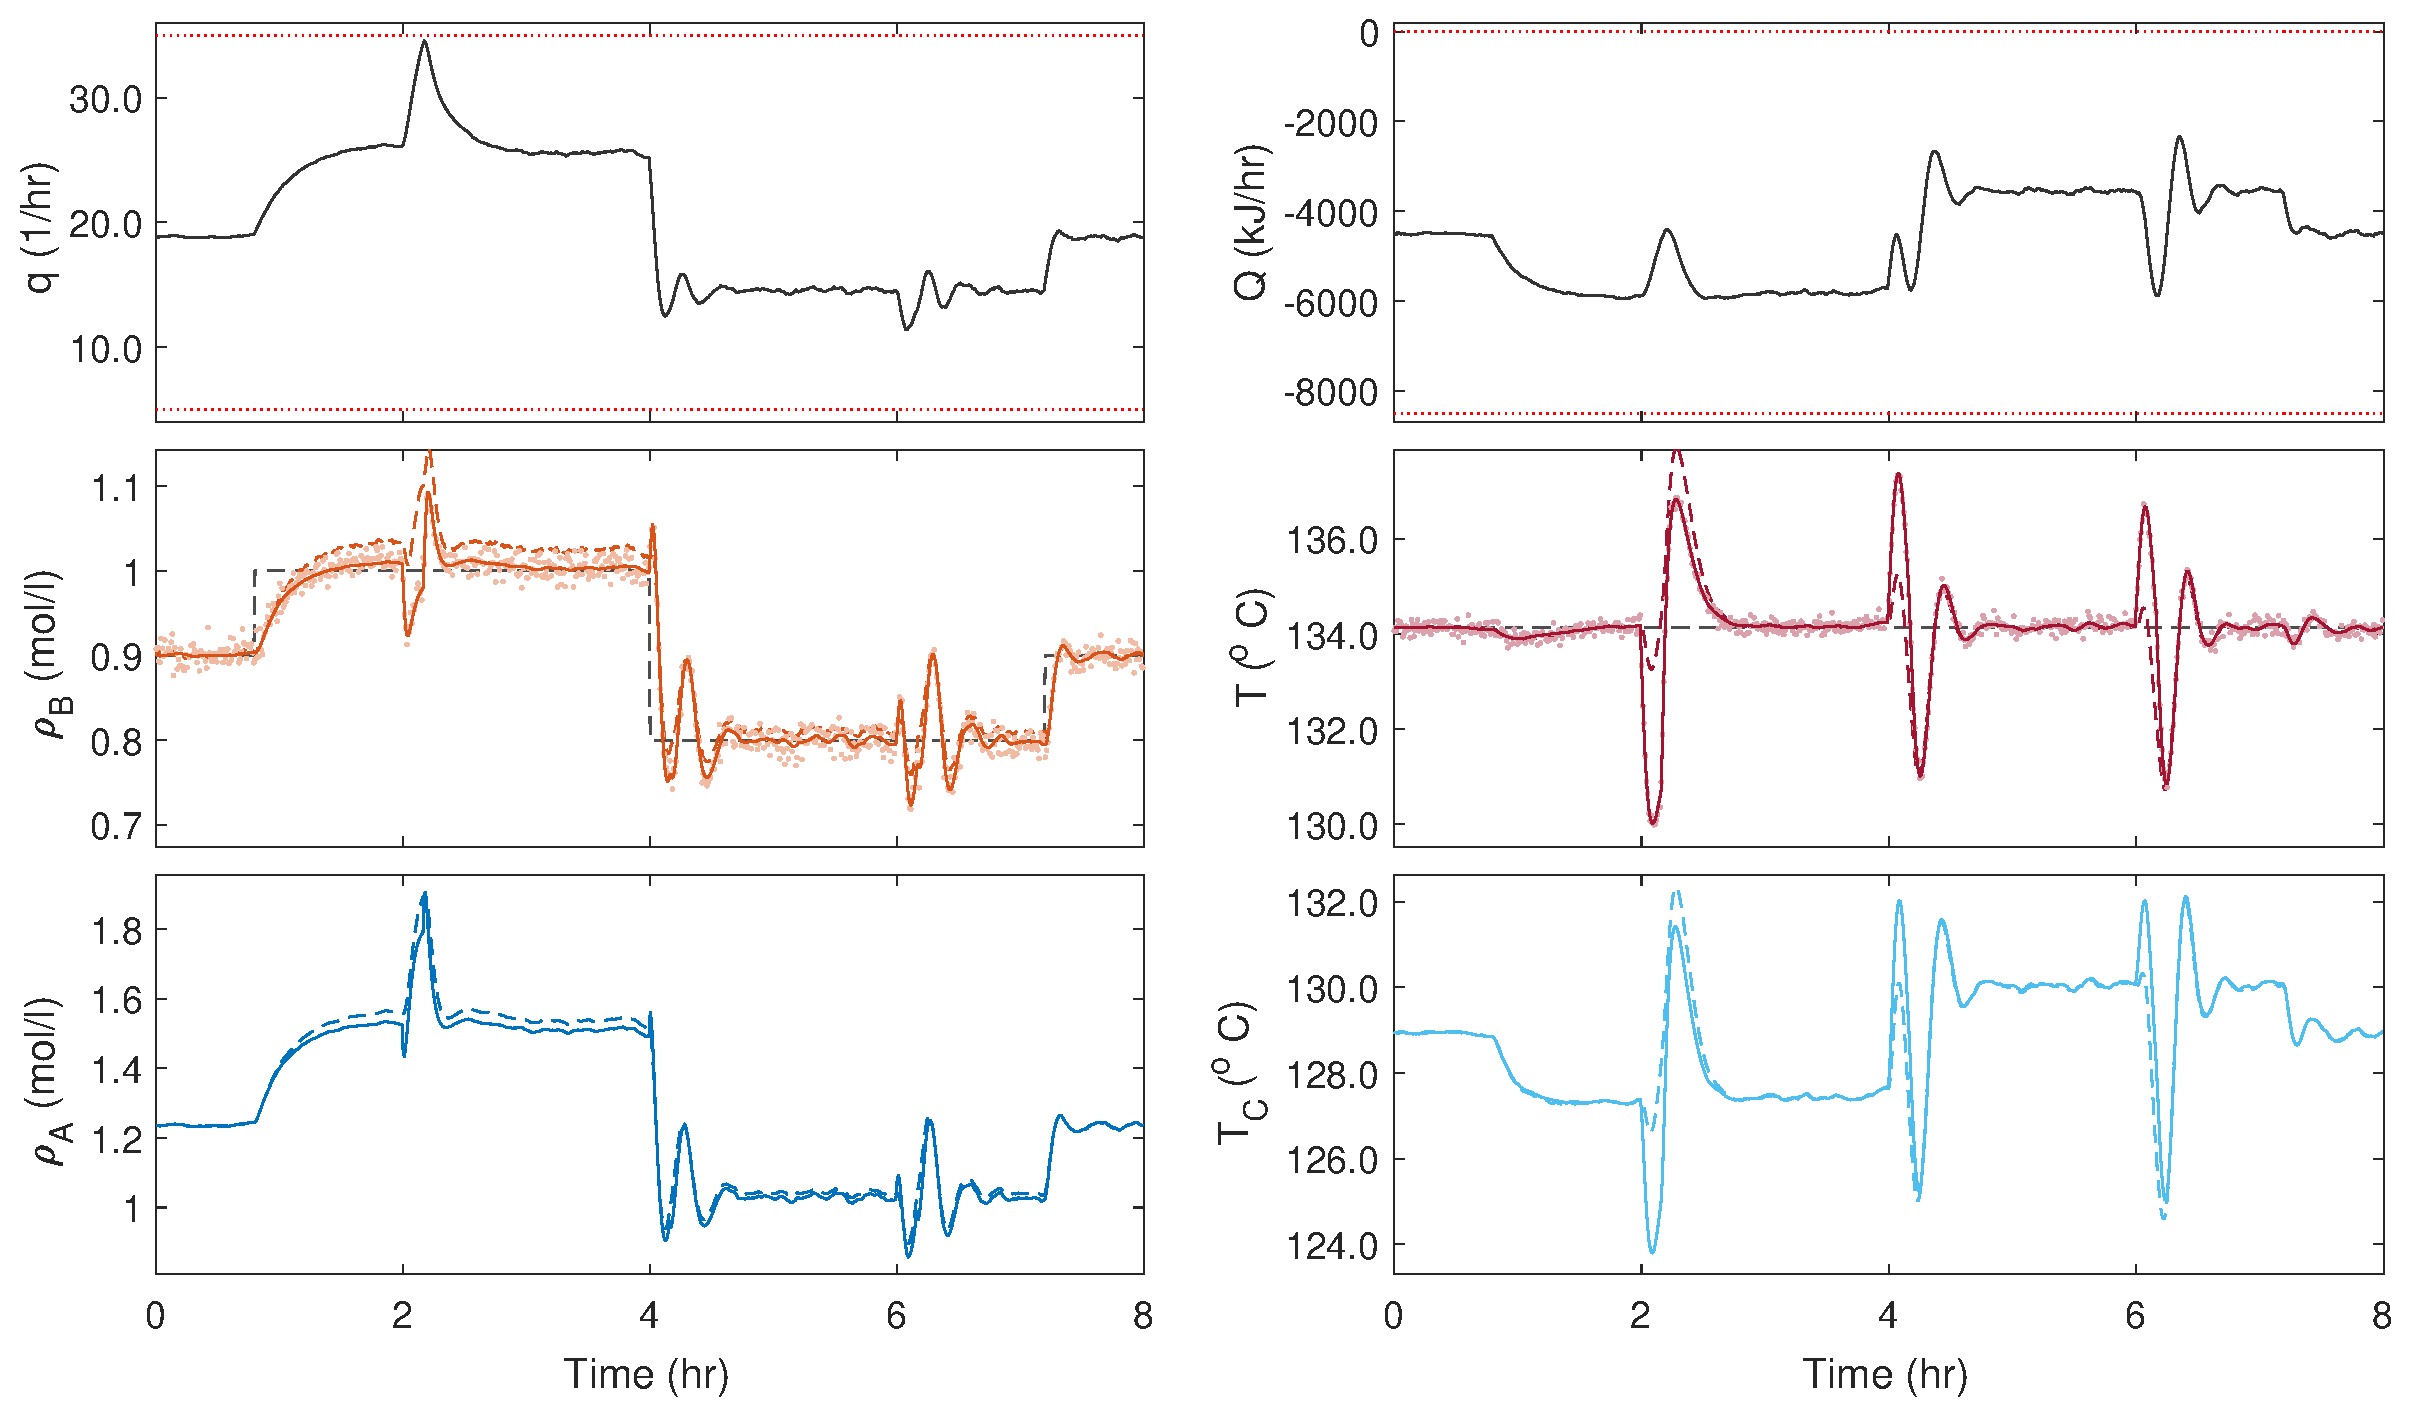
\includegraphics[width=\textwidth]{lqgi02}
\end{figure}

\end{frame}

%-------------------------------------------------------
% SECTION - Conclusion
%-------------------------------------------------------
\section{Conclusion}
%-------------------------------------------------------
\begin{frame}[c]{Conclusion}{}

\vskip0.25cm

\begin{itemize}
  \item We have demonstrated the theoretical foundations of optimal control and its application to a specific challenging problem. \vskip0.2cm
  
  \item There were noted some limitations:
  \begin{itemize}
    \item[$\circ$] The state estimator has not able to reconstruct the state information when far from the steady-state point. \vskip0.2cm
    
    \item[$\circ$] The integral action directly from noisy measurements demonstrated a concerning behavior. \vskip0.2cm
    
    \item[$\circ$] The optimization was performed in a unconstrained fashion, which is unpractical.
  \end{itemize} \vskip0.2cm
  
  \item This work opens the possibility of evaluating more advanced control and estimation techniques using the same mathematical framework. 
\end{itemize}

\end{frame}

%-------------------------------------------------------
%\begin{frame}[allowframebreaks] \small
%        \frametitle{References}
%        \bibliography{citations.bib}
%\end{frame}


%-------------------------------------------------------
%-- End Page
{\1
\begin{frame}[plain,noframenumbering]
  \center \Huge \textbf{Thank you!}       
  
  \includegraphics[scale=0.4]{corgi.jpg}
  
  Questions?
\end{frame}

%-------------------------------------------------------
\end{document}


%%---------------------Rascunho--------------------------
%\section{Titulo}
%\subsection{Subtitulo}
%%---------------------Rascunho--------------------------
%\begin{frame}{Titulo}{Subtitulo}
%
%\begin{block}{title}
% Say somethings \alert{new} 
%\end{block}
%
%\begin{itemize}
% \item TikZ\footnote{TikZ is a package for creating beautiful graphics. Have a look at these \chref{http://www.texample.net/tikz/examples/}{online examples} or the \chref{http://tug.ctan.org/tex-archive/graphics/pgf/base/doc/generic/pgf/pgfmanual.pdf}{pgf user manual}.}
%\end{itemize}
%
%\end{frame}
%%---------------------Rascunho--------------------------

%%%%%%%%%%%%%%%%%%%%%%%%%%%%%%%%%%%
%% Drafts:
%%%%%%%%%%%%%%%%%%%%%%%%%%%%%%%%%%%
%%%%% Figure:
% \begin{figure}[ht]
%   \centering
%   \includegraphics[trim={0cm 0cm 0cm 0cm},clip,scale=1]{nameFigure}
%   \caption{caption of the figure.}
%   \label{fig:nameFigure}
% \end{figure} \vskip0.25cm
%
%%%%% Equation:
% \begin{equation*} \label{eq:nameequation*}
% \begin{split}
%  X = 1 + 1
% \end{split}
% \end{equation*} \vskip0.25cm
%
%%%% Table:
% \begin{table}[hp]
%   \centering
%   \begin{tabular}{l | c c }
%   Principal & Coluna1 & Coluna2 \\
%   \hline 
%   ABC & 1 & 2 \\
%   DFG & 3 & 4 \\
%   HIJ & 5 & 6 \\
%   \end{tabular} 
%   \caption{caption of the table.}
%   \label{table:nameTable} 
% \end{table} \vskip0.25cm
